% !TeX spellcheck = cs_CZ
\documentclass[a4paper,hidelinks]{report}

\usepackage[utf8]{inputenc}
\usepackage[czech]{babel}
\usepackage{hyperref}
\usepackage{amsmath}
\usepackage{amsfonts}
\usepackage{amssymb}
\usepackage{listingsutf8}
\usepackage{xcolor}
\usepackage{inconsolata}
\usepackage{nameref}
\usepackage[a4paper,includeheadfoot,margin=3.5cm]{geometry}

%Vkladani source kodu
\lstdefinestyle{codeInput} { %
	language=C++,
	basicstyle=\ttfamily\footnotesize,
	numberstyle=\scriptsize,
	numbers=left,
	backgroundcolor=\color{gray!10},
	frame=single,
	keepspaces=true,  
	showspaces=false,
	showstringspaces=false,
	showtabs=false,
	tabsize=4,
	rulecolor=\color{black!30},
	escapeinside={\%*}{*)},
	breaklines=true,
	breakatwhitespace=true,
	framextopmargin=2pt,
	framexbottommargin=2pt,
	inputencoding=utf8/latin2,
	extendedchars=true,
	literate=
	{á}{{\'a}}1
	{í}{{\'i}}1
	{é}{{\'e}}1
	{ý}{{\'y}}1
	{ú}{{\'u}}1
	{ó}{{\'o}}1
	{ě}{{\v{e}}}1
	{š}{{\v{s}}}1
	{č}{{\v{c}}}1
	{ř}{{\v{r}}}1
	{ž}{{z}}1
	{ď}{{\v{d}}}1
	{ť}{{\v{t}}}1
	{ň}{{\v{n}}}1                
	{ů}{{\r{u}}}1
	{Á}{{\'A}}1
	{Í}{{\'I}}1
	{É}{{\'E}}1
	{Ý}{{\'Y}}1
	{Ú}{{\'U}}1
	{Ó}{{\'O}}1
	{Ě}{{\v{E}}}1
	{Š}{{\v{S}}}1
	{Č}{{\v{C}}}1
	{Ř}{{\v{R}}}1
	{Ž}{{\v{Z}}}1
	{Ď}{{\v{D}}}1
	{Ť}{{\v{T}}}1
	{Ň}{{\v{N}}}1                
	{Ů}{{\r{U}}}1    	
}
\lstset{style=codeInput}
\renewcommand{\lstlistingname}{Zdrojový kód}
\renewcommand{\lstlistlistingname}{Seznam zdrojových kódů}
\newcommand{\includecode}[3][default]
{\lstinputlisting[caption=#3 (#2),label=lst:#1, style=codeInput]{#2}}


\title{Simulace Sluneční soustavy}
\date{\today}
\author{Jan Waltl}



\usepackage{fancyhdr}
\setlength{\headheight}{15pt}

\pagestyle{fancy}
\renewcommand{\chaptermark}[1]{ \markboth{\thechapter \ #1}{} }
\renewcommand{\sectionmark}[1]{ \markright{\thesection \ #1} }

\fancyhf{}
\fancyfoot[C]{\thepage}
\fancyhead[L]{\textit{ \expandafter\MakeUppercase\expandafter{\leftmark}} }
\fancyhead[R]{\textit{ {\rightmark}} }

\fancypagestyle{plain}{ %
	\fancyhf{} % remove everything
	\renewcommand{\headrulewidth}{0pt} % remove lines as well
	\renewcommand{\footrulewidth}{0pt}
}

\begin{document}
	\begin{titlepage}
	\begin{center}
		\vspace*{8cm}
		\Huge{\textbf{Simulace Sluneční soustavy}}\\
		\vspace*{1cm}
		{\Large Dokumentace k zápočtovému programu pro předmět Programování I}\\
		\vfill
		
		\huge{Jan Waltl}\\
		\huge{12.Ledna 2017}
	\end{center}
\end{titlepage}
	

	\newpage
	\tableofcontents
	\lstlistoflistings
	\newpage
	% !TeX spellcheck = cs_CZ

\chapter*{Organizace dokumentu}
Tento text je organizován do následujících kapitol:
\begin{description}
	\item[\nameref{chap:uvod}] - Zadání zápočtového programu a teoretická část
	\item[\nameref{chap:implementace}] - Hlavní část dokumentace, které popisuje jak design celého programu, tak jednotlivých částí. Zaměřuje se na použité algoritmy a jejich implementaci včetně zdrojových kódů C++.
	Také zmiňuje možnosti rozšíření programu.
	\item[\nameref{chap:userGuide}] - Část popisující jak program spustit a jak s ním pracovat z neprogramátorského pohledu.
	
\end{description}
Text není nutné číst od začátku do konce, pro první spuštění by mělo stačit poslední kapitolu. Naopak, ale pro pochopení implementace RK4 metody je dobré vědět něco o numerické integraci a o co se vlastně program vůbec snaží. Což popisuje teoritická část v úvodní kapitole. Programátorská část vyžaduje znalost C++ a OpenGL, ale je zde snaha důležitější koncepty vysvětlit  i bez těchto znalostí. V tomto textu se nachází  zdrojové kódy s příklady, které jsou psány následujícím formátem:
\begin{lstlisting}
\caption{Text vystihující příklad (Název souboru)}
#include <iostream>

int main()
{
	std::cout<<"Hello World!\n";
	return 0;
}
\end{lstlisting}
Všechny další uvedené zdrojové kódy se nachází ve složce \texttt{Source/}, která
by měla být připojena k této dokumentaci. Z praktických důvodů \textbf{nemusí} být tyto soubory zkompilovatelné, popřípadě mohou být z části v pseudo-kódu. Také se \textbf{nejedná} o zdrojové kódy samotného programu. Primární účel je \textbf{popisný}. Ovšem často bude uvedený kód přímo nebo částečně odpovídat kódu někde uvnitř programu.
Zdrojové kódy samotného programu se přímo v tomto dokumentu nenachází, avšak jsou také součástí dokumentace a obsahují komentáře, které mohou stát za přečtení.
\vfill
\begin{center}
\textbf{	
Tato dokumentace spolu se zdrojovými kódy programu je dostupná na:\\
\texttt{https://bitbucket.org/Quimby/solar/src}\\
Popřípadě přímo stažitelná pomocí git:	\\
\texttt{https://Quimby@bitbucket.org/Quimby/solar.git}\\
V případě problému mne můžete kontaktovat na adrese: waltl.jan@gmail.com
}
\end{center}

	% !TeX spellcheck = cs_CZ

\chapter{Úvod}
\label{chap:uvod}

\section{Specifikace}
Program simuluje Sluneční soustavu za využití numerické integrace a Newtonova gravitačního zákona. Fyzikálně se jedná řešení problému n-těles - tzn. každé těleso gravitačně působí na všechna ostatní. Tento problém je velmi těžko řešitelný analytickým metodami pro větší n. Výpočetní síla počítačů spolu s metodami numerické integrace tak nabízí alternativní řešení tohoto problému.

\paragraph{}
Vstupem programu jsou strukturovaná data uložená v textovém souboru, která definují fyzikální veličiny simulované soustavy.Tedy polohy, rychlosti a hmotnosti simulovaných objektů. 
\paragraph{}
Výstup je 2D grafická reprezentace simulované soustavy v reálném čase. Uživatelské rozhraní dovoluje měnit rychlost a přesnost simulace. Dále zobrazuje užitečné informace, jako jsou aktuální pozice, rychlosti pro každý simulovaný objekt vzhledem k jiným objektům.
\paragraph{}
Při vývoji programu byl kladen co největší důraz na pozdější rozšířitelnost. Výsledný program tedy poskytuje několik simulačních metod a možností vstupů a výstupů. 

\section{Teorie}
\subsection{Analytický popis}
Newtonův Gravitační zákon (dále NGZ) popisuje vzájemné silové působení $ {F}_g $ dvou hmotných bodů
\footnote{Myšlené těleso, kde jeho veškerá hmotnost je soustředěna do jednoho místa - \textbf{hmotného bodu}. }
, kde výsledná síla je přitažlivá.

\begin{equation}
	{F}_g= \kappa \dfrac{m_1 m_2}{(\boldsymbol{x_1 - x_2})^2} 
\end{equation}
$ m_1,m_2 $ jsou hmotnosti obou bodů a $ \boldsymbol{x_1,x_2} $ jejich polohy.

Dále budeme pokládat simulované objekty za hmotné body, což je vzhledem k rozměrům hvězd, planet, měsíců a jejich vzdálenostem rozumná aproximace.

Nyní nám NGZ spolu s principem superpozice
\footnote{Princip superpozice říká, že výsledné silové účinky na těleso jsou dány součtem všech sil, které na něj působí.}
 a Newtonovým Zákonem síly \eqref{eq:sila} dává pro $ n $ těles následující \eqref{eq:soustava} soustavu  $ n $ obyčejných diferenciálních rovnic. 
 Kde neznámé $ \boldsymbol {x}_i, \boldsymbol{\ddot x}_i $ jsou vektory polohy, resp. zrychlení simulovaných těles. Mínus je zde kvůli přitažlivosti výsledné síly.
\begin{equation}
F= m  \boldsymbol {\ddot x}
\label{eq:sila}
\end{equation}
\begin{align}\label{eq:soustava}
\boldsymbol {\ddot x}_i = -\kappa \sum_{j=1,j \neq i}^{n}\dfrac{m_i\left( \boldsymbol{x_i}(t) - \boldsymbol{x_j}(t)\right)}
{\left( \boldsymbol{x_i}(t) - \boldsymbol{x_j}(t)\right) ^3} . 
\quad \text{pro } i=1 \dots n
\end{align}

Analytické řešení této soustavy rovnic by nám dalo možnost zjistit polohu, rychlost a zrychlení libovolného simulovaného objektu v libovolném čase na základě počátečních podmínek.
\paragraph{}
Bohužel vyřešit tuto soustavu je pro $ n=>3 $ velmi těžké.

\subsection{Numerické řešení}
\label{sec:numReseni}
Pokud se soustava nedá vyřešit analyticky, můžeme se alespoň pokusit získat aproximativní řešení. Numerická integrace využívá toho, že nemusí být těžké spočítat derivace v libovolném čase. Navíc to dnešní počítače dokáží udělat velmi rychle. Pokud tedy dokážeme zjistit derivaci v každém bodě, tak bychom mohli původní funkci zrekonstruovat pomocí těchto derivací. Např. můžeme výslednou funkci aproximovat úsečkami, kde jejich směrnice je derivace hledané funkce. Toto přesně dělá nejjednodušší integrační metoda - Eulerova explicitní metoda\eqref{eq:euler}.
Mějme jednoduchou soustavu rovnic \eqref{eq:ex} . Je vidět, že řešením je funkce$ y=e^t $, což se snadno ověří zpětnou derivací. 
\begin{align} \label{eq:ex}
\dot	y = y, y(0)=1
\end{align}
\begin{align} \label{eq:euler}
y(t+\Delta t) = y(t) + \Delta t . y'(t)
\end{align}
Zkusme tuto rovnici vyřešit numericky Eulerovou metodou \eqref{eq:euler}. 
Výsledné hodnoty pro různé  $ \Delta t $ jsou vykresleny na obrázku \ref{fig:euler} spolu s analytickým řešením.
Pro dostatečně malá  $ \Delta t $ dostáváme relativně přesné řešení.

Eulerova metoda se dá použít i k řešení naší soustavy \eqref{eq:soustava}, což je podrobněji popsáno u její implementace v sekci \ref{sec:implEuler}. Také další integrační metody - semi-implicitní Euler a RK4 jsou popsány u svých implementací
\ref{sec:implEuler} resp. \ref{sec:implRK4}.
\begin{figure}[p]
	\caption{Srovnání různých $ \Delta t $ pro přesnost Eulerovy metody}
	\label{fig:euler}
	\centering
	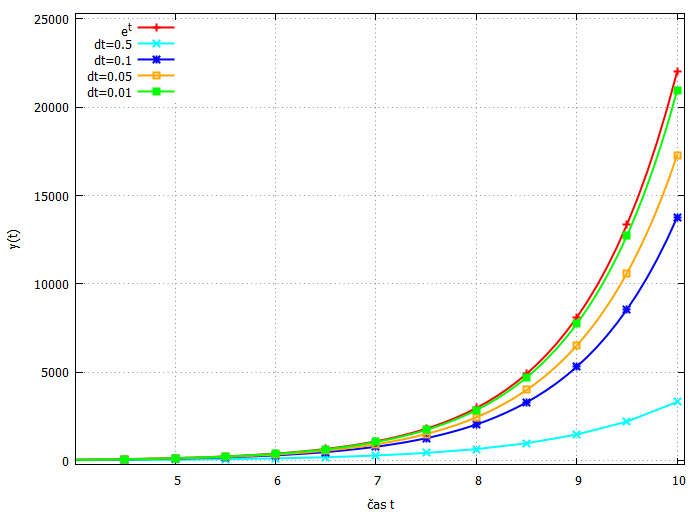
\includegraphics[width=\linewidth]{Figs/eulerTable}
\end{figure}










	% !TeX spellcheck = cs_CZ

\chapter{Návrh programu}
\label{chap:implementace}
Tato kapitola se zabývá návrhem programu - jak je celý program navržen a popisuje jeho hlavní třídu - \texttt{Simulation}. V rámci které si představíme \textbf{moduly}, které se objevují v dalších kapitolách.
Na úvod se podívejme jak by mohl vypadat jednoduchý \textbf{main.cpp} 

\includecode{Source/main.cpp}{Hlavní program}

Veškeré zdrojové kódy programu jsou zabaleny do jmenného prostoru \texttt{solar}. \texttt{Simulation} je hlavní třída, která se stará o celkový průběh simulace. Dále jsou zde vidět tři \textbf{moduly}, které jsou předány simulaci. Jejich detailní popis přijde později.

\texttt{Simulation} poté zajišťuje jejich vzájemnou spolupráci. Metoda \texttt{Simulation::Start()} následně spustí samotnou simulaci podle předepsaných parametrů.
Pokud někde nastane chyba, dojde k vyvolání výjimky v podobě třídy \texttt{solar::Exception}, popřípadě jiných výjimek z rodiny \texttt{std::exception}.


% !TeX spellcheck = cs_CZ

\section{Třída \texttt{Simulation}}
Je třída, která spojuje jednotlivé moduly do funkčního celku a zajišťuje průběh celé simulace, proto stojí za to se na ni podrobněji podívat. Nejprve se podíváme na veřejné rozhraní, které dovoluje simulaci ovládat. Poté nahlédneme i dovnitř abychom zjistili jak to celé funguje.
\subsection{Veřejné rozhraní}
Přibližně takto vypadají veřejné metody třídy \texttt{Simulation} :
\includecode{Source/simPublic.cpp}{Veřejně rozhraní \texttt{Simulation}}
\paragraph{Řídící funkce}
jsou funkce, které řídí spuštěnou simulaci. Jsou volány z modulů, ne z hlavního programu. Většinou se jedná o jednoduché funkce na 1-2 řádky, proto zde nejsou jednotlivě popsány, ale z jejich názvů je zřejmé co dělají. Případný náhled do zdrojových kódů by to měl objasnit.
\paragraph{Konstruktor}
očekává 3 moduly, které se budou v simulaci používat, podrobněji se na ně podíváme za okamžik. Zde jim také předá odkaz na simulovaná data.
\paragraph{Metoda \texttt{Start()}}
provádí samotnou simulaci. V této metodě stráví program většinu času, popíšeme ji podrobně v sekci \ref{sec:startMetoda} - vysvětlíme její teoretický návrh a implementaci, což také objasní její parametry.
\subsection{Moduly}
\label{sub:moduly}
Nyní si vysvětlíme co to \textbf{moduly} jsou a k čemu slouží.
Zkusme se zaměřit co by měla každá simulace vlastně udělat:
\begin{enumerate}
	\item \textbf{Načíst data}, bez nich není co simulovat. Což se dá popsat dvěma slovy a implementovat stovky způsoby. Takže by stálo za to, aby simulace uměla všechny.
	\item \textbf{Simulovat data}. Z teorie už víme, že také neexistuje pouze jedna integrační metoda, takže bychom chtěli mít na výběr. Určitě totiž není moc šťastné řešení zvolit jednu metodu a doufat, že bude stačit na všechny simulace.
	\item \textbf{Uložit data}. Také se chceme našimi výsledky pochlubit, ale kdyby nám je simulace pracně získala a hned zahodila, tak to půjde těžko. Ovšem stálo by za to umět je ukládat v různých formátech nebo třeba rovnou odeslat někam po internetu.
	\item \textbf{Prohlížet data}. Představme si situaci: 3:38 ráno, naše značně vylepšená verze simulace právě doběhla. Přidali jsme do ní nově objevené asteroidy u kterých chceme spočítat trajektorie. Z hrůzou ale zjistíme, že Země není tam kde má být, dokonce tam není vůbec! Co se mohlo asi stát? To je dobrá otázka, proto by mohlo být dobré mít přístup k datům i během simulace a třeba si je někam průběžně ukládat.
\end{enumerate}
Teď už víme, co by měla každá simulace zvládnout, ale je vidět, že toho má umět celkem hodně a ještě různými způsoby. Nejlepší tedy bude, aby se simulace(ve formě třídy \texttt{Simulation}) opravdu starala jen o to, aby tyto kroky proběhly, ale to jak přesně proběhnou přenecháme někomu jinému -\textbf{ modulům}, které se vyskytují ve 3 druzích:
\begin{description}
	\item[parser] obstarává výrobu vstupních dat. Také na konci simulace může výsledná data uložit.
	\item[simMethod] provádí simulaci dat např. pomocí nějaké numerické metody.
	\item[viewer] má přístup k datům za běhu simulace a může je např. zobrazovat na obrazovku nebo ukládat stranou.
\end{description}
Práci jsme rozdělili, simulace by to celé měla tedy organizovat, což se děje právě pomocí metody \texttt{Start()}, tak si ji pojďme představit.
\subsection{Návrh metody \texttt{Start()}}
\label{sec:startMetoda}
Takto nějak by mohla vypadat na první pohled rozumná implementace:
\includecode[startPseudo]{Source/startPseudo.cpp}{Návrh metody \texttt{Start()}}
Tato implementace by byla plně funkční, ale možná ne úplně vhodná pro náš cíl. Rádi bychom totiž prováděli a hlavně zobrazovali simulaci v reálném čase. 

Zde ale není žádné časování, \texttt{while} smyčka bude probíhat jak nejrychleji může, bez jakékoliv kontroly. Což není špatné, pokud chceme nechat program běžet a jen se pak podívat na výsledky, popřípadě mezivýsledky uložené někde v souborech. K tomu přesně slouží metoda \texttt{Simulation::StartNotTimed()}, která má přibližně výše uvedenou implementaci. 
\paragraph{Časování}
- K dosažení našeho cíle bude potřeba nějakým způsobem svázat reálný čas s tím simulovaným. Upravíme tedy předchozí příklad \ref{lst:startPseudo} následovně:
\includecode[startTimed]{Source/startPseudoTimed.cpp}
{Metoda \texttt{Start()} s časováním}
Pokud bychom chtěli opravdu simulaci v reálném čase, tak se v každém průběhu smyčkou podíváme jak dlouho trvala předchozí smyčka a tolik času musíme odsimulovat. Naivní implementace by byla předat přímo tento čas \texttt{acc} metodě, která se stará o simulaci. Tím bychom dostali nedeterministický algoritmus
\footnote{Algoritmus, který nemusí nutně vracet stejný výsledek při opakovaném volání se stejnými vstupními hodnotami.}.
Neboť trvání poslední smyčky je ovlivněno např. aktuálním vytížením počítače, což určitě není předvídatelné. A bohužel při počítaní s desetinnými čísly dochází k zaokrouhlovacím chybám, takže výsledek nezávisí pouze na vstupních datech, ale i na postupu výpočtu.

Řešení \footnote{Zdroj: \url{http://gafferongames.com/game-physics/fix-your-timestep/} (\today)}
je naštěstí jednoduché, budeme odečítat pevnou hodnotu \texttt{deltaT}.
A to tolikrát, abychom odsimulovali potřebný čas uložený v \texttt{acc}. Je pravda,
že nakonci nemusí platit $ acc=0 $, ale bude platit $ acc\leq deltaT $. A vzhledem k tomu, že \texttt{acc} si zachovává hodnotu mezi průběhy smyčkou, tak se zbytek času neztrácí, ale použije se v dalším průchodu. Takto dostaneme deterministický algoritmus.

\label{par:spiral}
Navíc máme objasněn první parametr - \textbf{deltaT(dt)} - základní časový krok simulace, který odpovídá $ \Delta t $ z teorie. Čím menší, tím je simulace přesnější, ale dochází k více voláním simulační metody, což může být potencionálně náročné na CPU.
Pro nízké hodnoty by se klidně mohlo snadno stát, že simulace přestane stíhat, tzn. že simulovat čas \texttt{deltaT} bude reálně trvat déle než \texttt{deltaT}. Např.
simulace \texttt{10ms} bude konstantně trvat \texttt{15ms}, v dalším průběhu smyčkou se tedy bude simulace snažit simulovat uběhlých \texttt{15ms}, což ale může trvat \texttt{22,5ms}. V dalším průběhu se tedy musí odsimulovat \texttt{22,5ms}...takový případ velmi rychle celý program odrovná. Proto je vhodné proměnnou \texttt{acc} omezit nějakou konstantou. Poté sice začne docházet ke zpožďování simulace, ale kontrolovaným způsobem.
\paragraph{Změna rychlosti} - Nyní bude naše simulace fungovat zcela správně a v reálném čase. Takže máme hotovo? Skoro, naše simulace je sice plně funkční, ale jediné co umí je předpovídat přítomnost a ještě jen s omezenou přesností. To není moc užitečné. Oběh Země kolem Slunce bude skutečně trvat 1 rok a Neptun to zvládne za 165 let. Tolik času nejspíše nemáme, proto by stálo za to najít nějaký způsob jak simulaci urychlit. Existují dva způsoby jak to udělat:
\begin{enumerate}
	\item Volat simulační metodu častěji. Například pro každý krok \texttt{deltaT} ji můžeme zavolat \texttt{rawMult}krát. Toto zrychlení jde na úkor výpočetního výkonu nutného k udržení této rychlosti, viz. předchozí odstavec.
	\item Volat simulační metodu s jiným \texttt{deltaT}, konkrétně s jeho \texttt{DTMult} násobkem. Tohoto zrychlení dosáhneme na úkor přesnosti. Protože předáváme větší $ \Delta t $ do simulační metody, což vede k menší přesnosti.
\end{enumerate}
Parametry \texttt{rawMult} a \texttt{DTMult} přesně odpovídají argumentům implementované verze metody \texttt{Simulation::Start()}.

Poslední parametr, který nebyl ještě vysvětlen je \texttt{maxSimTime}. Vzhledem k tomu, že volání funkce \texttt{Start()} může trvat velmi dlouho, tak je dobré nastavit horní limit, který garantuje přerušení smyčky po překročení zadaného času. \texttt{maxSimTime=0} znamená \texttt{maxSimTime=$ \infty $} ,tzn. simulace se přeruší pouze zavoláním funkce \texttt{Simulation::StopSimulation()}, kterou ale mohou volat pouze moduly, neboť jiné objekty nejsou při simulaci volány.
Popřípadě se přeruší vyvoláním nějaké vyjímky.

\subsection{Finální implementace metody \texttt{Start()}}
Poučeni z předchozí části upravíme naši rozpracovanou implementaci \ref{lst:startTimed} na \ref{lst:startFinal}. Což je už velmi podobné skutečné metodě použité v programu. Která navíc umožňuje simulaci pozastavit, krokovat a také pomocí C++ knihovny \texttt{chrono} implementuje opravdové časování, které zde bylo uvedeno spíše koncepčně.
\includecode[startFinal]{Source/startFinal.cpp}
{Finální verze \texttt{Simulation::Start()}}



\section{Výjimky}
Existují tři druhy výjimek, které program může vyvolat.
\begin{enumerate}
	\item Nejčastěji to bude výjimka v podobě třídy \texttt{Exception}, která dědí 
	z \texttt{std::runtime\_error} a tedy i \texttt{std::exception}. K této výjimce dojde zejména při chybě v otevírání/čtení souborů a inicializace knihoven, ale jedná se o hlavní třídu výjimek v tomto programu, takže je použita i v modulech pro hlášení chyb.
	\item Na výjimku v podobě třídy \texttt{GLError} můžeme narazit při chybě týkající se OpenGL - nepodařená inicializace, nedostatek paměti a podobně.
\item Výjimky dědící z \texttt{std::exception} - program využívá standardní C++ knihovny, které můžou potencionálně také vyvolat výjímky.
\end{enumerate}
Všechny tři druhy nabízí metodu \texttt{what()}, která vrátí krátký popis vyvolané výjimky.
	\chapter{Popis modulů}
Následující kapitoly se zabývají moduly popsanými v sekci \ref{sub:moduly}.
Nejprve si v této kapitole podrobně představíme každý ze 3 druhů modulů.
V dalších kapitolách se pak podíváme na konkrétní moduly, které byly implementovány, a ukážeme si příklad jak by se dal program rozšířit.

Ale ještě před představením modulů musíme udělat malou odbočku a definovat si pár tříd a pojmů, které moduly hojně využívají.
\paragraph{Třída \texttt{SystemUnit}}
je jednoduchá třída, ze které dědí veškeré moduly a která modulům zajišťuje spojení s rozhraním třídy \texttt{Simulation}.
\paragraph{Matematický aparát}
ve formě tříd \texttt{Vec2} a \texttt{Vec4} nabízí základní matematické operace s vektory jako je sčítání, odčítání a násobení skalárem. Také jsou k dispozici funkce
\texttt{length()} a \texttt{lengthsq()}, které počítají délku vektoru respektive její druhou mocninu.
\paragraph{struktura \texttt{Unit}}
je základní jednotka simulace. Jedná se o jeden simulovaný objekt, který má své vlastnosti - polohu, rychlost, hmotnost, jméno a barvu. Kde poslední dvě jsou dobrovolné a simulace se bez nich obejde, ale jsou zde kvůli zobrazování na obrazovku. Její definice je uvedena v následujícím zdrojovém kódu \ref{lst:unitDef}
\includecode[unitDef]{Source/unit.cpp}{Definice struktury \texttt{Unit}}
\paragraph{typ \texttt{simData\_t}} je \texttt{std::vector<T>} , kde \texttt{T} je \texttt{Unit}. Používá jako typ simulovaná data.
\section{Parser}
Parser se stará o výrobu vstupních dat, také má přístup k výsledným datům, která tak může uložit. Všechny třídy \textbf{parser} modulů musí dědit z abstraktní třídy \texttt{Parser}, jejíž přesná implementace je zde:
\includecode[parser]{Source/parser.cpp}{Abstraktní třída \texttt{Parser}} 
Hlavní funkce, kterou každý \textbf{parser} musí implementovat je \texttt{Load()} . Její úkol je libovolným způsobem načíst data a vrátit je ve formě \texttt{simData\_t}. Dále může přepsat metodu \texttt{Save()}, která je zavolána na konci simulace s výslednými daty.
\section{SimMethod}
Simulační metoda by měla zajistit samotnou simulaci. To jakým způsobem bude měnit data záleží pouze na ní. Může tedy použít libovolnou integrační metodu, ale pokud si bude házet imaginární kostkou, tak to bude fungovat také, ikdyž informační hodnota takové simulace je přinejlepším sporná. Podívejme se na přesnou definici abstraktní třídy \texttt{SimMethod}, která dává základ všem simulačním metodám
\includecode[simMethod]{Source/simMethod.cpp}{Abstraktní třída \texttt{SimMethod}}
Všechny zděděné moduly musí implementovat alespoň metodu \texttt{operator()()}, která provede jen krok simulace. Simulovaná si drží pomocí svého ukazatele.
Pokud potřebuje inicializovat své proměnné v závislosti na vstupních datech, tak může přepsat metodu \texttt{Prepare()}. Tato funkce je volána před startem simulace, ale po načtení dat, takže k ním má metoda už přístup. Což se může hodit pro metody, které potřebují znát velikost dat a podle toho si vytvořit dočasné proměnné.
\section{Viewer}
Poslední typ modulu - \textbf{viewer} - má přistup k datům za běhu simulace a  je  reprezentován abstraktní třídou \texttt{Viewer} jejíž definice je zde:
\includecode[viewer]{Source/viewer.cpp}{Abstraktní třída \texttt{Viewer}}
Každý \textbf{viewer} musí alespoň implementovat metodu \texttt{operator()()}, která je volána při každém průchodu smyčkou a má tedy vždy přístup k aktuálně simulovaným datům. Také, pokud potřebuje, může přepsat metodu \texttt{Prepare()}

	\chapter{FormattedFileParser}
Tento \textbf{parser} načítá strukturovaná data z textového souboru. 

Parser očekává základní SI jednotky - metry, sekundy, kilogramy. Ale výstupní \texttt{simData\_t} obsahuje objekty se vzdáleností v AU($ 1,5.10^9 $ m), časem v rocích(pozemské - 365 dní) a hmotností v násobcích hmotnosti Slunce($ 1,988435.10^{30} $ kg přesně). Důvod je ten, že hodnoty v těchto jednotkách jsou více normalizované a dochází k menším zaokrouhlovacím chybám.

\section{Struktura dat}
\label{sec:strukturaDat}
Začneme hned příkladem, takto by mohl vypadat správný vstupní soubor s daty:
\begin{lstlisting}
{ name<Sun>
color<1.0 0.88 0.0 1.0>
position<0.0 0.0>
velocity<0.0 0.0>
mass<1.98843e30> }

{ name<Earth>
color<0.17 0.63 0.83 1.0>
position< 149.6e9 0.0>
velocity<0 29800.0>
mass<5.9736e24> }

{ name<Moon>
color<0.2 0.2 0.2 1.0>
position< 150.0e9 0.0>
velocity<0 30822.0>
mass<7.3476e22> }
\end{lstlisting}
\texttt{FormattedFileParser} by z tohoto souboru vytvořil data obsahující 3 objekty pojmenované Sun, Earth, Moon s určitými vlastnostmi.

Každý objekt je popsán uvnitř páru složených závorek \textbf{\texttt{\{\}}}.
Všechny parametry objektu jsou dobrovolné, čili \lstinline|{}| je validní bezejmenný objekt, který se nachází v klidu na pozici \texttt{(0,0)} a má nulovou hmotnost. Pokud se ale parametr objeví, musí mít správný formát, který je obecně \texttt{název<hodnoty>}. Následuje přesný výčet a formát parametrů:
\paragraph{name$ < $jméno$ > $ } - jméno objektu. Jsou dovoleny pouze znaky ASCII, čili bez diakritiky. Pokud není uvedeno, pak je prázdné.
\paragraph{color$ < $R G B A$ > $} - barva objektu. Očekávají se 4 desetinná čísla v rozmezi od 0.0 do 1.0 oddělená mezerou představující barvu ve formátu RGBA. Pokud není uvedeno, pak je bíla.
\paragraph{velocity$ < $X Y$ > $} - počáteční rychlost objektu. Očekává dvě desetinná čísla oddělený mezerou reprezentující rychlost ve vodorovném a svislém směru. Nesmí zde být napsány fyzikální jednotky - tzn. \texttt{velocity$ < $10e2 m/s 8e3 m/s$ > $} \textbf{není} validní vstup. Ale implicitně by hodnoty měly být v m/s . Pokud není uvedeno, pak je (0,0).
\paragraph{position$ < $X Y$ > $} - počáteční pozice objektu. Identické s rychlostí, očekávají se hodnoty v metrech.
\paragraph{mass $ < $hmotnost$ > $ } - hmotnost objektu vyjádřená jedním desetinným číslem v kilogramech. Doporučení je zde také neuvádět jednotky, i když to bude fungovat, tak budou ignorovány. Pokud není uvedeno, pak je nulová hmotnost.
\paragraph{Dodatek k číslům} - jsou povolena jak celá, tak desetinná čísla. Je dovolena pouze desetinná tečka. Číslo 104.25 můžeme zapsat například takto: $ 104.25 ;\ 1.0425e2$.
\textbf{Parser} ovšem \textbf{neumí} aritmetiku, takže následující \textbf{není} validní vstup: $ 10425/100 ;\ 104 + 0.25 ;\ 1.0425 * 10^2 $.
\paragraph{}
\texttt{FormattedFileParser} je relativně shovívavý k formátování, takže následující příklad je ekvivalentní definice objektu \texttt{Sun} z předchozího příkladu.
\begin{lstlisting}
{ Main star of our Solar system has a name <Sun>. 
  It's color is usually <1.0 0.88 0.0 1.0 which means yellow in RGBA format.
  The Sun accounts for 99% mass of our entire system,
  which makes it nearly 330 thousand times heavier than Earth
  or to put it in another way it weights < 1.98843e30 kilograms>. }
\end{lstlisting}

\section{Detaily implementace}
Takto vypadá deklarace konstruktoru: \\
\lstinline|FormattedFileParser(const std::string& inputFileName,const std::string& outputFileName="");|\\
Parser tedy očekává vstupní a případně výstupní jméno souboru,\textbf{ včetně} cesty a přípony k souboru. Samotné načítání a ukládání probíhá v metodách \texttt{Load()} respektive \texttt{Save()}.

Na vlastní implementaci není koncepčně nic extra zajímavého. \texttt{Load()} načte celý soubor do \texttt{std::string} ve kterém si pak vždy najde dvojici \{\}, ve které se pokusí najít názvy parametrů. Pokud nějaký najde, pak k němu ještě najde nejbližší dvojici $ <> $  ve které poté očekává správné hodnoty. Tento jednoduchý způsob zajišťuje výše ukázanou flexibilitu formátování. Všechno ostatní, co by se v dokumentu mohlo nacházet(například komentáře) prostě ignoruje. 

\texttt{Save()} vytvoří soubor, pokud byl nějaký zadán, do kterého předaná data uloží. Což se děje podobným způsobem - každý parametr "zabalí" do správného formátu a převede do jednotek SI.
Při nekorektním vstupu, nemožnosti otevřít vstupní soubor nebo vytvořit soubor výstupní vyvolají funkce výjimku \texttt{Exception}.


\chapter{SolarParser}
\section{Popis}
Tento jednoduchý \textbf{parser} nedělá nic jiného, než že načte data o Sluneční soustavě, která má zabudována pevně ve své implementaci.
Momentálně se jedná o následující objekty:
\begin{enumerate}
	\item Hvězdy - Slunce
	\item Planety - Merkur, Venuše, Země, Mars, Jupiter, Saturn, Uran, Neptun
	\item Trpasličí planety - Pluto
	\item Měsíce - Měsíc, Phobos, Deimos, Io, Europa, Ganymed, Callisto
\end{enumerate}
Výstupní \texttt{simData\_t} obsahuje objekty se vzdáleností v AU($ 1,5.10^9 $ m), časem v rocích(pozemské - 365 dní) a hmotností v násobcích hmotnosti Slunce($ 1,988435.10^{30} $ kg přesně). Důvod je ten, že hodnoty v těchto jednotkách jsou více normalizované a dochází k menším zaokrouhlovacím chybám.

Také dokáže uložit výsledky simulace do formátovaného textového souboru stejného jako \texttt{FormattedFileParser} v předchozí kapitole
	\chapter{Implementované simulační metody}
\section{Explicitní Eulerova metoda}
\label{sec:explEuler}
Teorie za touto metodou byla popsána v úvodní kapitole. V naší soustavě 
\eqref{eq:soustava} ale máme i druhé derivace, proto si pomůžeme tím, že každá obyčejná diferenciální rovnice $ n $-tého stupně se dá převést na $ n $ rovnic prvního stupně, takže nám vzniknou dvě rovnice \eqref{eq:secDer23} na které aplikujeme Eulerovu metodu \eqref{eq:euler} a dostaneme numerické řešení v podobě \eqref{eq:soustavaExplEuler}
\begin{subequations}
	\label{eq:secDer23}
	\begin{align}
	\label{eq:secDer2}
	\boldsymbol{\dot x}(t)&= \boldsymbol{v}(t) \\
	\label{eq:secDer3}
	\boldsymbol{\dot v}(t)&=- \Delta t . \kappa \sum_{j=1,j \neq i}^{n}\dfrac{m_j}
	{\left[ \boldsymbol{x_i}(t) - \boldsymbol{x_j}(t)\right] ^3} . 
	\left[ \boldsymbol{x_i}(t) - \boldsymbol{x_j}(t)\right] 
	\end{align}
\end{subequations}
\begin{subequations}\label{eq:soustavaExplEuler}
	\begin{align}
	\boldsymbol {x}_i(t+\Delta t)& =\boldsymbol{{x}}_i(t)  +\boldsymbol {v}_i(t)\\
	\boldsymbol {v}_i(t+\Delta t) &=\boldsymbol{{v}}_i(t)  - \Delta t . \kappa \sum_{j=1,j \neq i}^{n}\dfrac{m_j}
	{\left[ \boldsymbol{x_i}(t) - \boldsymbol{x_j}(t)\right] ^3} . 
	\left[ \boldsymbol{x_i}(t) - \boldsymbol{x_j}(t)\right] 
	\end{align}
\end{subequations}
Implementace této metody by mohla vypadat například jako \ref{lst:methodExplicitEuler}. Ve dvojité smyčce tedy projdeme všechny dvojice a spočítáme nové rychlosti a poté ještě upravíme polohu. Potřebujeme si v dočasné proměnné uchovat původní rychlost a polohu v čase $ t $. Netvrdím, že se jedná o nejefektivnější algoritmus, ale tvrdím, že na tom nezáleží, protože tato metoda není moc vhodná pro náš problém, protože vyžaduje velmi malé $ \Delta t $ a je vždy nestabilní - viz. kapitola \ref{chap:compMethods}.
\includecode[methodExplicitEuler]{Source/explicitEuler.cpp}
{Explicitní Eulerova metoda}

\section{SemiImplicitEuler}
\label{sec:implEuler}
\subsection{Teorie}
V minulé části jsme se věnovali explictiní Eulerově metodě, ještě existuje implicitní verze \eqref{eq:implicitEuler}, která je teoreticky shodná s explicitní až na to, že derivaci vyčíslíme v čase $t + \Delta t $.
\begin{align} \label{eq:implicitEuler}
y(t+\Delta t) = y(t) + \Delta t . y'(t+\Delta t)
\end{align}
Nyní se podívejme jak bychom řešili jednoduchou diferenciální rovnici \eqref{eq:secDer}, kterou si stejně jako v minulé části upravíme na dvě rovnice \eqref{eq:secExDer2} a \eqref{eq:secExDer3}
\begin{align} \label{eq:secDer}
\ddot{x}(t) &= k.x(t) \quad \\
\text{s počátečními podmínkami:}& \quad x(0)=x_0, \quad \dot{x}(0)=v_0\nonumber
\end{align}
\begin{subequations}
	\label{eq:secExDer23}
	\begin{align}
	\label{eq:secExDer2}
	\dot x(t)&= v(t) \\
	\label{eq:secExDer3}
	\dot v(t)&=k.x(t) 
	\end{align}
\end{subequations}
Tak zkusme vyřešit nejdříve \eqref{eq:secExDer3} a použijeme implicitní verzi. Tím dostaneme rovnici \eqref{eq:secExDer4}. Teď použijeme stejný postup i na \eqref{eq:secExDer2} a výsledkem je \eqref{eq:secExDer5}. Nyní stačí dosadit první rovnici do druhé a po úpravě dostaneme hledaný výsledek, pak ho ještě dosadíme zpět do první a tím máme obě proměnné explicitně vyjádřené rovnicemi \eqref{eq:secExDer6} a \eqref{eq:secExDer7}.
\begin{align}
\label{eq:secExDer4}
 v(t + \Delta t)&=v(t) + \Delta t . \dot{v}(t + \Delta t)  
 =  v(t) + \Delta t . k.x(t + \Delta t)\\
 \label{eq:secExDer5}
 x(t+\Delta t) &= x(t) + \Delta t. \dot{x}(t+ \Delta t) = x(t) + \Delta t.v(t+ \Delta t) \\
 \label{eq:secExDer6}
 x(t+\Delta t) &= x(t) + \Delta t. \left[ v(t) + \Delta t . k.x(t + \Delta)\right]  \nonumber\\
 x(t+\Delta t) - \Delta t^2 .k.x(t+\Delta t) &=x(t) + \Delta t.  v(t) \nonumber\\
  x(t+\Delta t) &= \frac{x(t) + \Delta t.  v(t)}{1 - \Delta t^2 k}\\
  \label{eq:secExDer7}
   v(t + \Delta t)&=v(t) + \Delta t . k.\frac{x(t) + \Delta t.  v(t)}{1 - \Delta t^2 k} = \frac{\Delta t .k. x(t) + v(t)}{1-\Delta t^2 k}
\end{align}
To sice dalo určitou práci, ale dostali jsme správné řešení. Na pravé straně  máme proměnné pouze v čase $ t $ takže je známe z předchozího kroku. V implementaci je nejspíše efektivnější spočítat jen jednu a druhou pomocí \eqref{eq:secExDer4} nebo \eqref{eq:secExDer5}.

Naše soustava rovnic \eqref{eq:soustava} je nápadně podobná předchozí rovnici \eqref{eq:secDer}, což samozřejmě není náhoda. Pokud se ale nyní budeme stejný postup snažit aplikovat na naší soustavu rovnic, tak zjistíme, že to nebude fungovat. Narazíme totiž na to, že po dosazení obou rovnic nebudeme schopni explicitně vyjádřit $ x(t + \Delta t) $. Bohužel toto je daň za vyšší stabilitu implicitních metod - nutnost vyřešení další rovnice. V našem případě bychom museli použít numerické řešení i pro samotnou rovnici, což dělat nebudeme.

Místo toho použijeme semi-implicitní Eulerovu metodu. Místo dvojitého použití implicitní metody použijeme implicitní pro \eqref{eq:secDer8} a explicitní verzi pro \eqref{eq:secDer7} . Explicitní verze nám dovolí snadno spočítat $ v(t + \Delta t) $ neboť hodnoty v čase $ t $ už známe. Tím jsme ale získali i potřebnou hodnotu $ v(t + \Delta t) $ pro implicitní verzi druhé rovnice. Vlastně jsme z obou metod vzali to nejlepší - jednoduchost explicitní a větší stabilitu implicitní metody. Výsledný mix je metoda, která je jednoduchá na implementaci a relativně přesná pro naše účely. Srovnání explicitní, implicitní a semi-implicitní Eulerovy metody se věnuje kapitola \ref{chap:compMethods}
\begin{align}
\label{eq:secDer7}
v(t + \Delta t)&=v(t) + \Delta t . \dot{v}(t)\\
\label{eq:secDer8}
x(t+\Delta t) &= x(t) + \Delta t. \dot{x}(t + \Delta t) = x(t) + \Delta t.v(t + \Delta t)\quad
\end{align}
Naše finální soustava \eqref{eq:soustava} po použití této metody bude \eqref{eq:soustavaEuler} pro $ i=1 \dots N $
\begin{subequations}\label{eq:soustavaEuler}
\begin{align}
\boldsymbol {v}_i(t+\Delta t) &=\boldsymbol{{v}}_i(t)  - \Delta t . \kappa \sum_{j=1,j \neq i}^{n}\dfrac{m_j}
{\left[ \boldsymbol{x_i}(t) - \boldsymbol{x_j}(t)\right] ^3} . 
\left[ \boldsymbol{x_i}(t) - \boldsymbol{x_j}(t)\right] \\
\boldsymbol {x}_i(t+\Delta t)& =\boldsymbol{{x}}_i(t)  +\boldsymbol {v}_i(t+\Delta t)
\end{align}
\end{subequations}
\subsection{Implementace}
Když jsme si metodu pracně teoreticky popsali, tak se nyní podívejme na to, jak bychom ji implementovali do našeho programu. Implementace by mohla vypadat například jako v \ref{lst:methodEuler}
\includecode[methodEuler]{Source/euler.cpp}
{Semi-implicitní Eulerova metoda}
Soustava \eqref{eq:soustavaEuler} nám říká, že nejdříve musíme spočítat novou rychlost objektu, která ale záleží na polohách všech ostatních. Takže musíme projít všechny dvojice, což nám zajistí dvojitá \texttt{for} smyčka. Dále potřebuje sečíst sumu, což se děje právě ve vnitřní smyčce. Protože je silové působení symetrické a pouze opačného směru, tak to můžeme udělat vždy pro celou dvojici najednou.
Vnitřní smyčka nám spočítala správnou rychlost levého(\texttt{left}) objektu.
Můžeme tedy spočítat jeho novou polohu dle \eqref{eq:soustavaEuler}.

Důležité je ověřit, že opravdu počítáme správně veličiny a hlavně ve správný čas. A skutečně je to takto správně, protože pozice levého objektu už v dalších smyčkách není použita a zároveň vnitřní smyčka opravdu správně spočítala novou rychlost levého objektu, kde pozice pravých objektů ještě upraveny nebyly a jsou tedy v čase $ t $.


\section{RK4}
\label{sec:implRK4}
\subsection{Teorie}
\paragraph{}

V předchozí sekci jsme implementovali Eulerovu metodu. Tato metoda lokálně aproximovala hledanou funkci pomocí úseček. Což znamenalo, že jsme na intervalu $ \left[ t,t+\Delta t\right]  $ považovali derivaci za konstantu, a to samozřejmě nemusí být pravda a v našem případě ani není. Proto se podívejme na další metodu -  \textbf{Runge-Kutta čtvrtého řádu(RK4)} . Která počítá derivaci vícekrát v různých bodech časového intervalu $ \left[ t,t+\Delta t\right]  $ a poté provede vážený průměr ze kterého poté dopočítá novou hodnotu hledané funkce. Mějme rovnici \eqref{eq:RK4Ex}, pak RK4 dává numerické řešení ve formě rovnice \eqref{eq:RK4Ex2}. Jedná se o explicitní verzi, ke které existuje ještě varianta implicitní, kterou ale implementovat nebudeme.
\begin{align}
\label{eq:RK4Ex}
\boldsymbol{\dot y} (t) &= \boldsymbol{f}(\boldsymbol{y},t) \quad \boldsymbol{y}(0)=\boldsymbol{y_0}\\
\label{eq:RK4Ex2}
\boldsymbol{y}(t + \Delta t) &= \boldsymbol{y}(t) + \frac{\Delta t}{6}\left[ \boldsymbol{k}_1 + 2\boldsymbol{k}_2 + 2\boldsymbol{k}_3 + \boldsymbol{ k}_4\right] \\
\boldsymbol{k}_1 &= \boldsymbol{f}(\boldsymbol{y}(t),t)\nonumber\\
\boldsymbol{k}_2 &= \boldsymbol{f}(\boldsymbol{y}(t) + \Delta t\frac{\boldsymbol{k}_1}{2}, t+\frac{\Delta t}{2})\nonumber \\
\boldsymbol{k}_3 &= \boldsymbol{f}(\boldsymbol{y}(t) + \Delta t\frac{\boldsymbol{k}_2}{2}, t+\frac{\Delta t}{2})\nonumber \\
\boldsymbol{k}_4 &= \boldsymbol{f}(\boldsymbol{y}(t) + \Delta t. \boldsymbol{k}_3, t+\Delta t)\nonumber
\end{align}

Zkusme tedy tuto metodu aplikovat na naši soustavu \eqref{eq:soustava}. Použijeme stejný trik jako u Eulerovy metody \eqref{eq:secDer23} a z jedné rovnice druhého řádu uděláme dvě rovnice první řádu \eqref{eq:RK4}.
\begin{subequations}
	\label{eq:RK4}
	\begin{align}
	\label{eq:RK4pos}
	\dot{\boldsymbol{x}}(t)&=\boldsymbol{v}(t)\\
	\label{eq:RK4vel}
	\dot{\boldsymbol{v}}(t)&=-  \kappa \sum_{j=1,j \neq i}^{n}\dfrac{m_j}
	{\left[ \boldsymbol{x_i}(t) - \boldsymbol{x_j}(t)\right] ^3} . 
	\left[ \boldsymbol{x_i}(t) - \boldsymbol{x_j}(t)\right] 
	\end{align}
\end{subequations}
Ve výše zmíněném popisu RK4 \eqref{eq:RK4Ex} se žádná soustava na první pohled nevyskytuje, v zadání je pouze jedna funkce, ale vektorová. Proto definujme následující vektorovou funkci \eqref{eq:defU}. Pak vlastně řešíme rovnici \eqref{eq:defUder} s neznámou funkcí $ \boldsymbol{u}(t) $, na kterou přesně aplikujeme RK4.
\begin{align}
	\label{eq:defU}
	\boldsymbol{u}(t) &:= (\boldsymbol{x}(t),\boldsymbol{v}(t)) \equiv(x_x,x_y,v_x,v_y)(t)\\
	\label{eq:defUder}
	 \boldsymbol{\dot{u}}(t)&=(\dot{\boldsymbol{x}}(t),\dot{\boldsymbol{v}}(t))=
	 (\boldsymbol{v}(t), -\kappa \sum_{j=1,j \neq i}^{n}\dfrac{m_j\left[ \boldsymbol{x_i}(t) - \boldsymbol{x_j}(t)\right]}
	 {\left[ \boldsymbol{x_i}(t) - \boldsymbol{x_j}(t)\right] ^3}
	  )
\end{align}


\subsection{Implementace}
Nyní se budeme věnovat tomu, jak by se RK4 dalo zakomponovat do našeho programu.
Implementace už je trochu delší, ale podrobně si ji vysvětlíme.
\includecode[method RK4]{Source/RK4.cpp}
{Runge-Kutta integrační metoda}

Nejprve si všimneme, že naše soustava nezávisí přímo na čase, ale pouze na aktuální poloze a rychlosti. Budeme také už potřebovat nějaké dočasné proměnné, konkrétně si budeme ukládat všechny 4 koeficienty pro každý objekt. Dále si ještě vytvoříme proměnnou, kam budeme ukládat mezistavy kroku - \texttt{temps}. Neboť pro spočítání $ k_{i+1} $ potřebujeme znát $ k_{i} $.

Nyní se zaměřme na funkci \texttt{computeKx}, která počítá koeficient. Z toho jak jsou koeficienty definované je musíme počítat postupně, protože do koeficientu $ k_i  $ dosazujeme stav $ y(t)+mult. \Delta t . k_{i-1} $.
Výpočet koeficientu je vlastně jen jeden krok explicitní Eulerovy metody. Akorát nepočítáme přímo simulovaná data, ale právě jen dočasný stav. Také nepočítáme posun o $ \Delta t $ ale o jeho násobek - \texttt{mult} argument.

Explicitní metodu už máme vymyšlenou z minula, tomu také odpovídá implementace.
Na konci nám ale ještě přibude finální integrace dat pomocí \eqref{eq:RK4Ex2}.
A také musíme nastavit dočasné proměnné pro další volání funkce.
	\chapter{IMGuiViewer}
Je grafický \textbf{viewer}, který zobrazuje simulované objekty ve 2D a dovoluje ovládání simulace pomocí uživatelského rozhraní. Jeho implementace je rozdělena do relativně velkého množství tříd a využívá externí knihovny, které si představíme jako první.

\section{Třída \texttt{OpenGLBackend} a GLFW\&GLEW}
Tento program používá k vykreslování grafiky OpenGL, tato třída má na starosti jeho správnou inicializaci. Používá k tomu knihovnu \textbf{GLFW} a \textbf{GLEW}.
GLFW\footnote{http://www.glfw.org/} poskytuje funkce k vytvoření okna do kterého může poté OpenGL kreslit.
GLEW\footnote{http://glew.sourceforge.net/} se stará o získání OpenGL funkcí, které se musí načíst za běhu aplikace z konkrétních grafických ovladačů na cílovém počítači.
Přesná implementace je dostupná ve zdrojových kódech programu. Ale jedná se ve větší míře o přepsání doporučené implementace na stránkách obou knihoven.

\subsection{Třída \texttt{Shader}}
Slouží pro jednoduší vytváření OpenGL shaderů, tedy malých programů určených pro grafickou kartu, které říkají jak má interpretovat a kreslit předaná data.
\subsection{Řešení OpenGL chyb} 
OpenGL samo nemá výjimky a chyby sděluje pomocí funkce \texttt{glGetError()}, která vrací typ chyby pokud nějaká nastala. Proto byla vytvořena funkce \texttt{ThrowOnError}, která zavolá \texttt{glGetError()} a při jakékoliv chybě vyvolá výjimku právě v podobě třídy \texttt{GLError}.
\subsection{Úvod do OpenGL}
... NewFrame, že se prekresluje frame a díky vnější smyčce to funguje...
\subsection{Třída \texttt{ImGuiBackend} a ImGui}
Se stará o integraci knihovny \textbf{ImGui}\footnote{https://github.com/ocornut/imgui}, která poskytuje nástroje k vytvoření uživatelského rozhraní.
Její implementace byla také vytvořena na základě příkladů uvedených na stránkách knihovny a dokumentace v souborech \texttt{imgui.h} a \texttt{imgui.cpp}. 
Pojďme si v rychlosti představit nějaké funkce knihovny, abychom pak lépe pochopili její použití při tvorbě uživatelského rozhraní.

\textbf{ImGui} je psáno v C++ ale z vnějšího pohledu vypadá spíše jako C, nejsou zde žádné složité třídy a většina prvků je z vnějšku bezstavová. To, co je tím myšleno vysvětluje následující kód
*Draw Button, draw if pressed, 
*C printf-like text
*Draw window
*Výjimka jsou comboboxy,selectables - stav si musíme uchovávat sami.
*Příklady použítí, že je skoro bezestavová - jen to co je mezi newframe a render,

\section{Kreslení simulace}
Nyní představíme pár tříd, které se starají o vykreslení samotných simulovaných dat
\subsection{třída \texttt{OMSAR}}
\texttt{OMSAR}(z Offset-Move-Scale-Aspect-Ratio) slouží k transformaci mezi souřadnou soustavou simulovaných dat a normalizovanými souřadnicemi, které využívá OpenGL. Jedná se o třídu ze které mají ostatní třídy zdědit sadu funkcí, která právě popsanou transformaci zajišťuje. Pomocí této třídy je také zajištěno posouvání obrazovky a přibližování/oddalování, což se děje pomocí dvou proměnných \texttt{Vec2 offset}(posouvání) a \texttt{scale}(přibližování). Tyto dvě proměnné využívají ostatní třídy, aby si správně posunuly vykreslované prvky na obrazovku.
\subsection{třídy \texttt{CircleBuffer} a \texttt{SimDataDrawer}} 
První jmenovaná třída umí vykreslit kruh o zadaném poloměru do středu obrazovky. K tomu využívá prvky OpenGL - konkrétně \textbf{buffery}. Pro posouvání se musí použít správný \textbf{shader}.
 
Druhá jmenovaná třída vykresluje data, kde jednomu objektu odpovídá právě jeden \texttt{CircleBuffer} - kruh. Data vykresluje pomocí funkce \texttt{Draw()}, která zajišťuje správný \textbf{shader} a využívá právě \texttt{OMSAR} k určení polohy jednotlivých kruhů.
\subsection{třída \texttt{UnitTrail}}
Při simulaci Sluneční soustavy by se nám hodilo nejen vidět aktuální polohu všech objektů, ale i jejich minulé polohy. Tato třída vykresluje lomenou čáru, která pak slouží jako \uv{stopa} za simulovaným objektem. Ideálně bychom tedy chtěli mít pouze funkci, která přidá další bod lomené čáry a to aktuální polohu.O to jak bude stopa uložena a kreslena se starat nechceme. Samozřejmě bude omezená maximální délku, ale to si má také ohlídat sama. Ještě pro úplnost existuje funkce \texttt{Clear}, která uloženou čáru smaže.

\paragraph{Algoritmus}Využijeme toho, že OpenGL přímo podporuje kreslení lomených čar, stačí zadat množinu bodů a ono samo mezi nimi vykreslí lomenou čáru. Navíc použijeme indexované vykreslování, tedy, že řekneme OpenGL v jakém pořadí má body vykreslit, což ve výsledku zajistí, že se celá množina bodů nemusí ležet ve správném pořadí a při přidávání bodů ji nebude nutné celou posunout.

Mějme dvě pole - bodů velikosti \textbf{n} a indexů o délce \textbf{2n}.
Dále máme objekt, který postupně projde body \textbf{A-B-C-D-E-F}. Tak pokud za ním chceme vykreslit stopu(lomenou čáru) o maximálně \textbf{n} bodech. Pak vytvoříme funkci \texttt{Push(Bod b)}, která umístí předaný bod do pole bodů. Pokud už je plné tak začne přepisovat body od začátku. Pole indexů vyplníme čísly od \textbf{1} do \textbf{n} dvakrát. Obrázek \ref{fig:lineTrail} popisuje jak bude algoritmus pro náš objekt fungovat při projití všech bodů, kde v každém bodě zavoláme \texttt{Push(bod)} a délka stopy je \textbf{n=3}. Pokud jsou v obrázku černě vyplněné např. indexy 2,3,1. Tak to znamená, že se vykreslí přímka v pořadí: \lstinline|body[2],body[3],body[1]|(což je napsáno vpravo).

Takže jediné co nám stačí je vytvořit indexové pole a posouvat odkud se má číst. Poté můžeme body v bufferu přepisovat, ale nemusíme celé pole posouvat při každém vložení.
\\

\textbf{Poznámka:}\textit{Teoreticky žádné indexy nepotřebujeme a mohli bychom kreslit vždy pouze úsečku. Ale zavolání jednoho vykreslení je v OpenGL relativně drahé, proto je lepší kreslit co nejvíce dat jedním příkazem. Proto také máme jeden kontinuální buffer pro body a jeden pro indexy. Tento algoritmus tedy považuji za kompromis mezi rychlostí a čitelností kódu. Teoreticky také stačí index buffer o velikosti \textbf{n} a pak čáru kreslit na dvakrát, protože je v bufferu buď uložená kontinuálně a nebo rozložená do dvou částí. Což by byla rozumná paměťová optimalizace, ale indexy zas tolik místa nezabírají a navíc existuje pouze jeden globální buffer pro všechny instance třídy \texttt{UnitTrail} neboť je jen pro čtení.}
\begin{figure}
	\caption{Kreslení stopy za objektem procházejícím body A-B-C-D-E-F}
	\label{fig:lineTrail} 
	\centering
	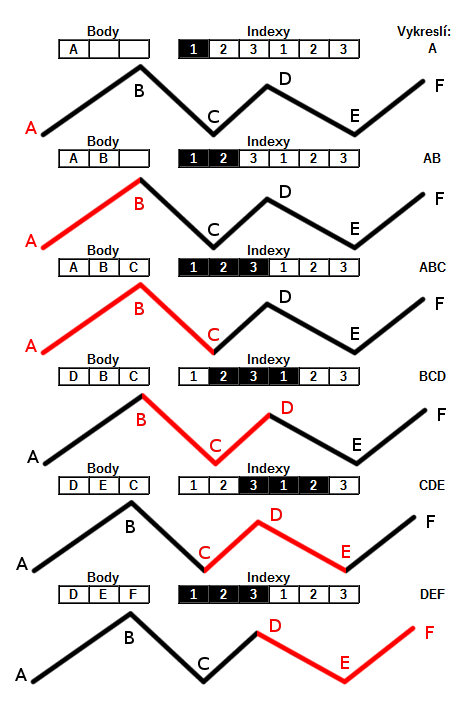
\includegraphics[width=0.5\linewidth]{Figs/LineTrail}
\end{figure}
\subsection{Třída \texttt{LineTrailsDrawer}}
Tato třída vytvoří pro každý simulovaný objekt jednu \texttt{UnitTrail}, do kterých pak periodicky ukládá jejich pozice a také všechny stopy vykresluje, k čemuž používá správný shader a informace z \texttt{OMSAR}. Nabízí také pár kontrolních funkcí jako selektivní mazání/vypínání/zapínání stop pro jednotlivé objekty.

\section{Kreslení uživatelského rozhraní}
Celé uživatelské rozhraní využívá plně knihovnu \textbf{ImGui} a je rozděleno do několika následujících souborů.
\begin{description}
	\item[MouseControls] Skupina funkcí, která implementuje ovládání pomocí myši. Tedy posouvání obrazovky a přibližování/oddalování.
	\item[SimProperties] Skupina funkcí, které vykreslují okno s informacemi o simulaci a také dovolují simulaci ovládat.
	\item[Visuals] Skupina funkcí, která vykresluje okno s ovládáním grafických prvků, tedy momentálně pouze kreslení stop za objekty. Dovoluje stopy selektivně vypínat/zapínat pro všechy objekty.
	\item[UnitsProperties] třída, která vykresluje okno, které zobrazuje fyzikální informace o vybraném objektu.
\end{description}
Koncepčně na těchto třídách není nic moc zajímavého. Ze zdrojových kódů a názvů funkcí v nich je celkem jasné co dělají.


	\chapter{Rozšířitelnost a vylepšení}

Pokud jste už zkusili výsledný program spustit a samou radostí nad skvělou simulací vám něco uniklo a vy jste v panice začali hledat tlačítko na vrácení o krok zpět, tak jste zjistili, že tam žádné není. Simulace ve výchozím stavu neprovádí žádné cachování/ukládání mezivýsledků, takže se nelze vrátit zpět. Což je určitě užitečné rozšíření, ale my zkusíme něco trochu jiného - \textbf{přehrávač simulací}.
Přehrávač by měl umět zaznamenat probíhající simulaci a poté ji přehrát jako video, tedy včetně přeskakování na libovolné místo simulace a zrychlení/zpomalení přehrávání.

\section{Návrh přehrávače}
Jak by se takový přehrávač dal implementovat?
Co kdybychom vytvořili následující třídy:
\begin{enumerate}
	\item Třída \texttt{ViewAndRecord}, která se chová jako libovolný jiný \texttt{viewer}, ale navíc si "tajně" zaznamenává simulaci do souboru. 
	\item Trojice tříd \texttt{ReplayerParser}, \texttt{ReplayerMethod} a \texttt{ReplayerViewer} které by se starali o samotné přehrávání simulace.
	\item Dvoji tříd \texttt{RecordedSimulation} a \texttt{ReplayedSimulation} které vše zabalují do funkčního celku.
\end{enumerate}
Celý přehrávač je plně funkční a součástí výsledného programu, proto si zde všechny koncepty alespoň přibližně představíme.
Navíc se v původním programu vlastně koncepčně vůbec nic nezměnilo, vše plyne z flexibility modulů.
\\
\\
\textbf{Poznámka autora:}  \textit{Při pohledu do git
	\footnote{Viz. Uživatelská příručka}
historie projektu zjistíte, že je to samozřejmě lež - měnilo se skoro všechno. Za prvé se úplně rozebral \texttt{ImGuiViewer} - vytáhly se z něj jednotlivé části, které se umístily do svých vlastních tříd. \textbf{Viewer} se poté z nich znovu sestavil zpět. Výsledná podoba je ta uvedená v dokumentaci, ve které jsou jednotlivé části co nejvíce nezávislé a hlavně znovupoužitelné.
Za druhé se zpřehlednilo rozhraní třídy \texttt{Simulation}, hlavně práce s časem, kdy se přešlo od desetinných čísel k celočíselné reprezentaci, která netrpí na zaokrouhlování.
Obě úpravy nebyly nutné z hlediska původní funkčnosti, ale už při implementaci se mi návrh moc nelíbil(zvlášť GUI bylo nepřehledné), každopádně cíl byl nejdřív dostat funkční kód a pak ho zkrášlovat dle potřeby.
Ve výsledku se velká část uživatelského rozhraní pro \texttt{ImGuiViewer} použila i pro \texttt{ReplayerViewer}, což by předtím vedlo na ošklivé {\small CTRL+C a  CTRL+V}}.

\section{Zaznamenání simulace}
Ideálně bychom chtěli zaznamenat jakoukoliv simulaci, což můžeme udělat například následujícím způsobem:
\includecode[recording]{Source/recording.cpp}
{Návrh jak by se simulace dala zaznamenávat}
Díky modulům se zaznamenávání simulace docílí velmi jednoduše, protože jediné co musíme změnit je, že \uv{zabalíme} zvolený \textbf{viewer} do třídy \texttt{ViewerAndRecord} a poté ho předáme jako obyčejný \textbf{viewer} simulaci. Při běhu simulace bude pak volán \texttt{ViewerAndRecord}, který ale v rámci své \texttt{operator()()} také zavolá předaný \textbf{viewer} a navíc si bude na pozadí ukládat probíhající simulaci.

Čili takto jednoduše jsme docílili zaznamenání skoro libovolné simulace.
Co se týče formátu záznamu, tak se jedná o binární soubor, kde jeho přesná specifikace je popsána u zdrojových kódů v souboru \texttt{FileFormats/ReplayerFile.txt}.
Zaznamenávání je nastaveno tak, že jeden simulovaný krok odpovídá jednomu záznamu. Odsimulovaný čas si \texttt{ViewAndRecord} snadno zjistí pomocí funkce \texttt{simTime Simulation::GetSimTime()}.
Slovo \uv{skoro} na začátku odstavce odkazuje na to, že tento postup selže, pokud někdo bude měnit simulovaný čas pomocí \texttt{void Simulation::SetSimTime(simTime)}, což ale klasická simulace dělat nepotřebuje.


\section{Přehrávání}
Přehrávání docílíme tím, že simulaci budeme podstrkovat data, která si přečteme ze souboru se zaznamenanou simulací místo toho abychom je simulovali sami. Tento podvod bude zajišťovat právě třída \texttt{ReplayerMethod}. Technicky potřebujeme ještě \textbf{parser} - \texttt{ReplayerParser}, ale ten jediné co udělá je, že přečte první data ze stejného souboru a tím vytvoří \texttt{simData\_t}, která se od tohoto modulu očekávají. Pro zobrazení použijeme třídu \texttt{ReplayerViewer}, která využívá pracně vytvořené části z modulu \texttt{IMGuiViewer}. Navíc ještě přidává okno, které obsahuje ovládání přehrávání. Mezi funkce patří slíbené zpomalení/zrychlení přehrávání a také přeskočení do libovolného bodu záznamu. 

Jak to funguje? \texttt{ReplayerMethod} si přečte aktuální odsimulovaný čas, podle toho si v souboru najde záznam, který tomu má odpovídat a simulovaná data prostě změní podle tohoto záznamu. Ve skutečnosti ještě provede lineární interpolaci mezi dvěma záznamy, aby byl výsledek plynulejší při menších rychlostech. \texttt{ReplayerMethod} je poté zobrazí bez ohledu na jejich původ. Pokud potřebujeme přehrávání zpomalit, tak využijeme parametru \texttt{DTMultiplier}. A pokud chceme přeskočit někam jinam, tak změníme odsimulovaný čas pomocí \texttt{void Simulation::SetSimTime(simTime)}.

Tím máme vlastně všechny moduly určené, ale nutit uživatele k tomu aby je vytvářel sám je zbytečné. Proto se o toto stará třída \texttt{ReplayedSim}, která obsahuje samotnou simulaci, které předá potřebné moduly.
\section{Vylepšení a opravy}
V průběhu prací na programu jsem si vedl v souboru plán toho, na čem budu pracovat, časem se tam objevily různé věci, které se do finálního programu z různých důvodů nedostaly, proto je zmíním alespoň zde jako možná vylepšení a také opravy toho co nebylo ještě opraveno.

\begin{description}
	\item[Fyzikální jednotky] Asi hlavní věc, která programu momentálně chybí je nějaký ucelený systém fyzikálních jednotek. \texttt{simData\_t} obsahují pouze data, takže záleží na dohodě mezi moduly, v jakém formátu tyto data jsou. Což je samozřejmě nepraktické. Řešení by bylo změnit \texttt{simData\_t} z vektoru na alespoň strukturu, která by měla pomocné proměnné označující v jakých jednotkách data jsou. Například pomocí \textbf{enum}, popřípadě rovnou dvojice (čitatel, jmenovatel) pro převod do jednotek SI, stejně jako používá knihovna \texttt{std::chrono}.
	\item[Šablony pro vektory] Není potřeba nic extra složitého, ale stálo by za to mít obecný vektor pro libovolný počet prvků a hlavně pro libovolná data. V samotném vektoru není potřeba moc změn, jen přepsání \textbf{double} na \textbf{T} a přidání pár \textbf{template}, ale tím se rozbije valná většina kódu všude možně v programu, takže oprava je zdlouhavá a otravná.
	Každopádně obecné vektory by se na pár místech v kódu hodily - GUI, OpenGL.
	\item[Rozšíření do 3D] Pokud bychom měli obecný vektor, tak rozšíření do 3D už je skoro hotové, protože integrační metody fungují pro libovolnou dimenzi a kód v nich by se skoro přepisovat nemusel. Do vykreslení pak stačí přidat projekční matici a \uv{trackball} pro ovládání myší a bylo by hotovo.
	\item[Zaznamenávání podle \texttt{simMethod}] Momentálně je zaznamenávání simulace vázáno na \textbf{viewer}, což je nepraktické, protože data opravdu mění \textbf{simMethod} a může se stát díky časování, že simulace proběhne vícekrát a my se na mezidata nepodíváme. Toto hodnotím jako špatný návrh, který by se měl opravit. Momentálně je to spíše opravdu jako zaznamenávání obrazovky při přehrávání simulace. Když se přehrávaná simulace bude sekat,tak bude zasekaný i záznam, přitom by stačilo si ukládat samotnou simulaci a ne obrazovku se simulací.
	\item[Zpomalení přehrávané simulace] Pokud byla simulace zaznamenána v reálném čase, tedy $ DTmult=RawMult=1 $, tak nejde při přehrávání zpomalit, protože to k tomu využívá právě \texttt{DTmult}, který ale nemůže být menší než 1. Bohužel mě nenapadá uspokojivé řešení, ale situace by neměla nastat moc často, protože simulaci přítomnosti moc často nechceme. Navíc zpomalení neposkytuje žádné nové informace, jen dochází k lineární interpolaci mezi záznamy, aby i pomalejší přehrávání bylo plynulé.
	\item[Lepší než lineární interpolace] Momentálně přehrávání používá lineární interpolaci polohy, což není moc přesné. Dala by se interpolovat i rychlost a zohlednit to v poloze. Aby se např. obíhající měsíc pohyboval po oblouku a ne po přímce mezi záznamy.
	
	Jde to vidět například u měsíců Jupitera, které jsou stabilní pro RK4 i při vysokém simulačním kroku a při zpomaleném přehrávání se pohybují spíše po mnohoúhelníku než kružnici. Ale toto je jen vizuální detail, nic podstatného.
	
	\item[Lepší GUI] Uživatelské rozhraní je podle mého názoru dostatečné, ale knihovna \textbf{ImGui} je celkem rozsáhlá a nabízí podporu např. pro kreslení grafů. Takže by se dal program rozšířit o velmi detailní statistiky - např. rozložení hmotnosti a rychlostí v soustavě. A také celkové energie systému, se kterou by se dala sledovat chyba integrační metody, protože energie uzavřeného systému je konstantní. Také by si GUI zasloužilo lepší podporu pro různé velikosti okna, což momentálně funguje, ale není to moc hezky napsané.
	\item[Nějaké zajímavé integrační metody] Toto by neměl být vůbec problém, kvůli tomu přesně existují moduly. Původně jsme chtěl přidat alespoň jednu vícekrokovou metodu, ale upřímně se mi už nechce, program je už dostatečně velký. Ale zajímalo by mě, jak si vedou v poměru přesnost/výkon hlavně vzhledem k RK4.
	Také využití OpenGL shaderů k simulaci by bylo zajímavý, což by mohlo dovolit simulovat více objektů.
	\item[Komprese zaznamenaných simulací] Aktuálně nedochází k žádné kompresi záznamu, takže po 5 minutách simulace při zaznamenání každých 10ms má soubor velikost kolem 15MB (30 tisíc záznamů). Avšak těžko říct kolik se bude dát reálně ušetřit, 7Zip tento konkrétní soubor zkomprimuje na 12MB pomocí algoritmu LZMA2, což není nic extra. 
	
	Ale malý krok simulace nevolíme většinou kvůli nutnosti znát polohu v každém čase, ale kvůli přesnosti simulace a samotných výsledků, takže řešením by byla možnost změnit ve třídě \texttt{ViewAndRecord} jak často se má zaznamenávat, což je úprava na pár řádku (změna \texttt{timeStep} a \texttt{multiplier} v .cpp by měla stačit).
	
\end{description}
	\chapter{Porovnání integračních metod}
V této kapitole alespoň zběžně porovnáme implementované integrační metody. Protože potencionálního uživatele by mohlo zajímat, kterou metodu by měl použít pro co nejpřesnější ale i nejrychlejší výsledek.

Srovnání bude probíhat nejdříve na případu kruhového pohybu. Důvod je ten, že je to podobný případ jako gravitace a také už pro něj máme vyřešenou implicitní verzi Eulerovy metody. Budeme hodnotit přesnost, stabilitu v závislost na $ \Delta t $ a výpočetní složitost.

V dalších sekcích už nebudeme metody znovu vysvětlovat, pouze se odkážeme na odpovídající kapitoly.

\section{Kruhový pohyb}
Zdrojové kódy použitých metod, které byly použity k získání dat, jsou dostupné v souboru \texttt{Source/stabilita.cpp}. Dále je zde soubor \texttt{plot.gp} pomocí něhož a gnuplotu
\footnote{\url{http://www.gnuplot.info/}}
 vznikly všechny obrázky.
\subsection{Teorie}
Pohyb po kružnici v rovině můžeme zapsat rovnicí \eqref{eq:kruh}, kde $\omega$ je úhlová rychlost. Což je také řešení diferenciální rovnice \eqref{eq:kruhDif}
\begin{align}
\label{eq:kruh}
\boldsymbol{u}(t) &= (x,y)(t)=(cos(\omega t),sin(\omega t))\\
\label{eq:kruhDif}
\ddot{\boldsymbol{u}}(t)&=-\omega^2u(t) \quad \boldsymbol{u}(0)=(1,0) \quad \dot{\boldsymbol{u}}(0)=(0,1)
\end{align}
V dalších částech zvolíme $ \omega = 1 $.
\subsection{Explicitní Euler}
Explicitní Eulerovu metodu jsme si představili v úvodní teorii \ref{sec:numReseni}. Zde jen připomeneme, že si opět rovnici \eqref{eq:kruhDif} rozdělíme na dvě rovnice prvního řádu a integrujeme je samostatně. Výsledky jsou zobrazeny v grafu na obrázku \ref{fig:explicitEuler}, z něhož je vidět, že explicitní metoda diverguje od správného řešení pro libovolné $ \Delta t $ Což není moc překvapivé, protože považuje derivaci na integračním oboru za konstantní, což je na počátku tečna procházející bodem (1,0) a tím dojde vždy k posunu směrem ven z kružnice. Takže tato metoda není moc vhodná pro naši simulaci, proto není ani implementována.
\begin{figure}
	\caption{Explicitní Eulerova metoda $ t\in [0,10] $}
	\label{fig:explicitEuler} 
	\centering
	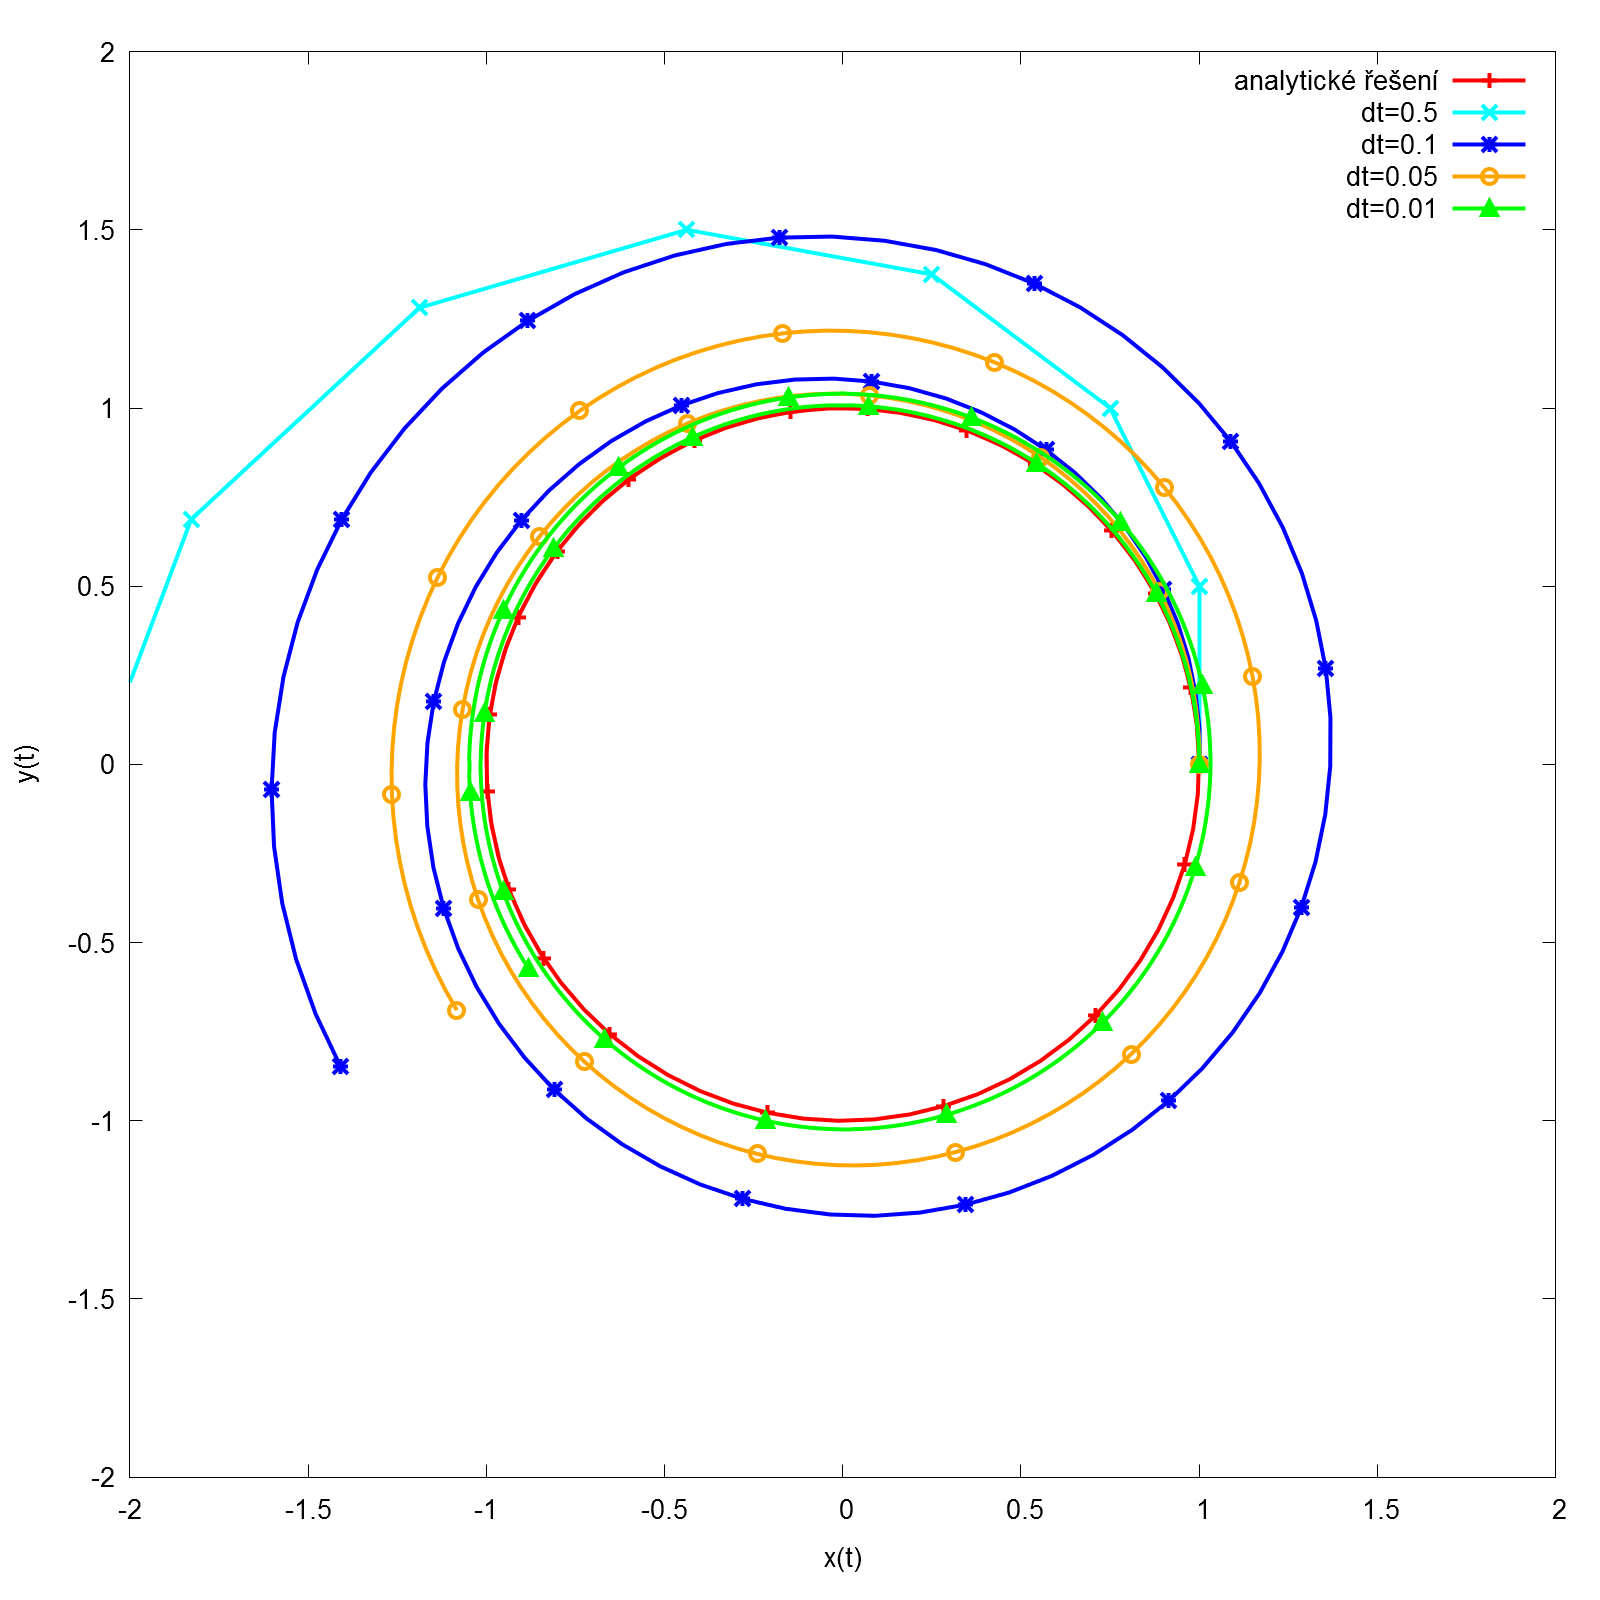
\includegraphics[width=\linewidth]{Figs/explicitEuler}
\end{figure}
\subsection{Implicitní Euler}
Implicitní Eulerova metoda byla ukázána v části \ref{sec:implEuler} i s řešením jedné rovnice \eqref{eq:implicitEuler}, které můžeme použít, neboť platí, že $ k=-\omega^2 $. 
Bohužel ani tato metoda není ideální jak ukazuje obrázek \ref{fig:implicitEuler}. Dochází zde k opačnému jevu, což je způsobeno tím, že integrace probíhá po tečně v čase $ t+\Delta t $, což vede k posunu směrem do kružnice. Implicitní metoda nebyla použita, protože se z naší soustavy \eqref{eq:soustava} nedá jednoduše vyjádřit a stejně by nepřinesla užitečné výsledky.
\begin{figure}
	\caption{Implicitní Eulerova metoda $ t\in [0,10] $}
	\label{fig:implicitEuler} 
	\centering
	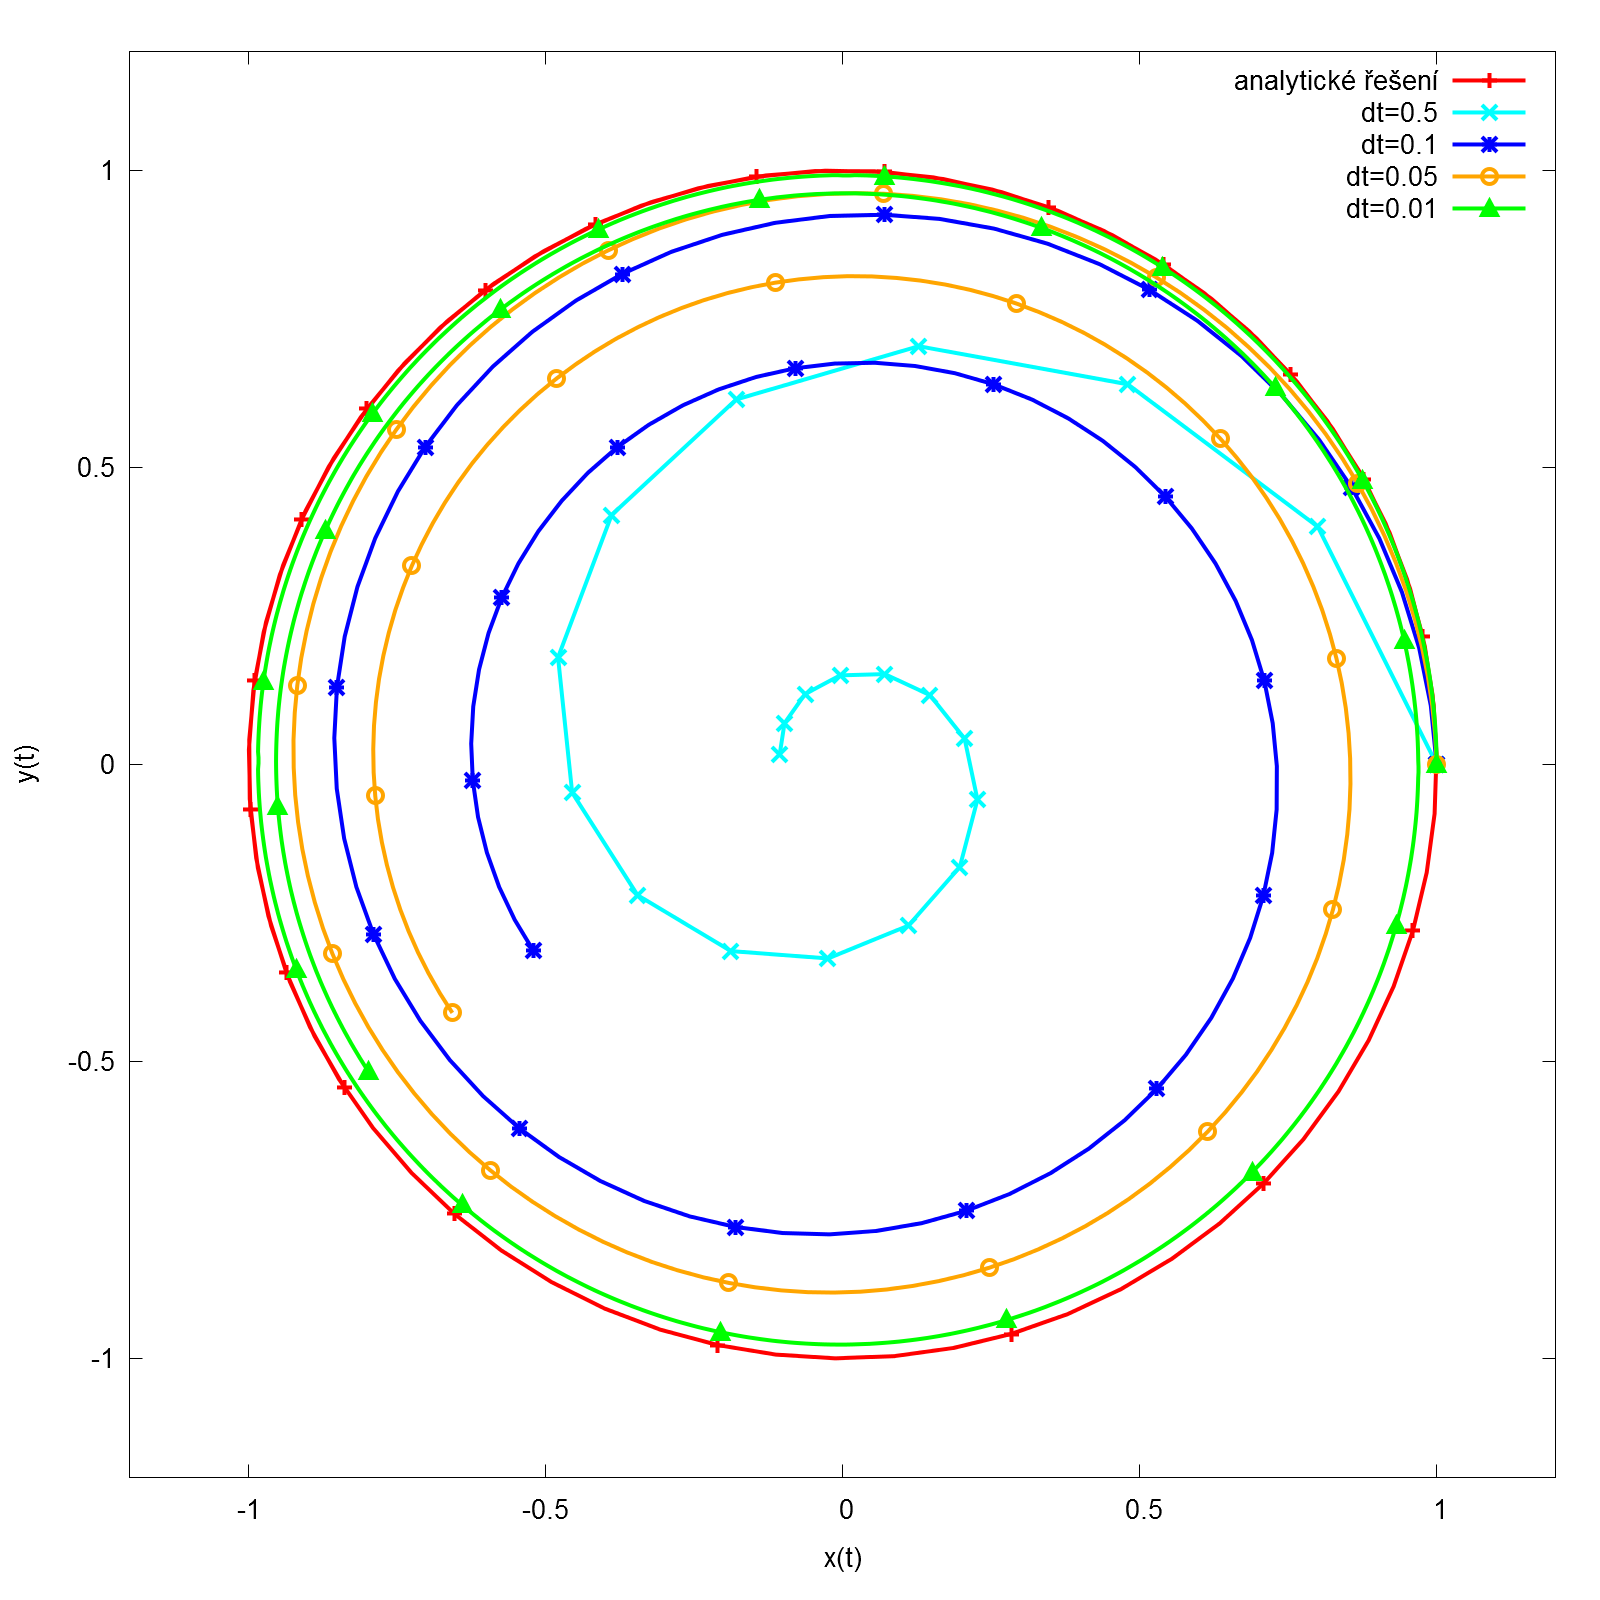
\includegraphics[width=\linewidth]{Figs/implicitEuler}
\end{figure}
\subsection{Semi-implicitní Euler}
Tato metoda je navrhnuta také v části \ref{sec:implEuler} jako jednodušší řešení implicitní verze. Z obrázků \ref{fig:semiImplEuler} a \ref{fig:semiImplEulerStab} je vidět, že je tato metoda navíc stabilní i pro větší $ \Delta t $, ale pro ně není už moc přesná.

\begin{figure}
	\caption{Semi-implicitní Eulerova metoda $ t\in [0,10] $}
	\label{fig:semiImplEuler} 
	\centering
	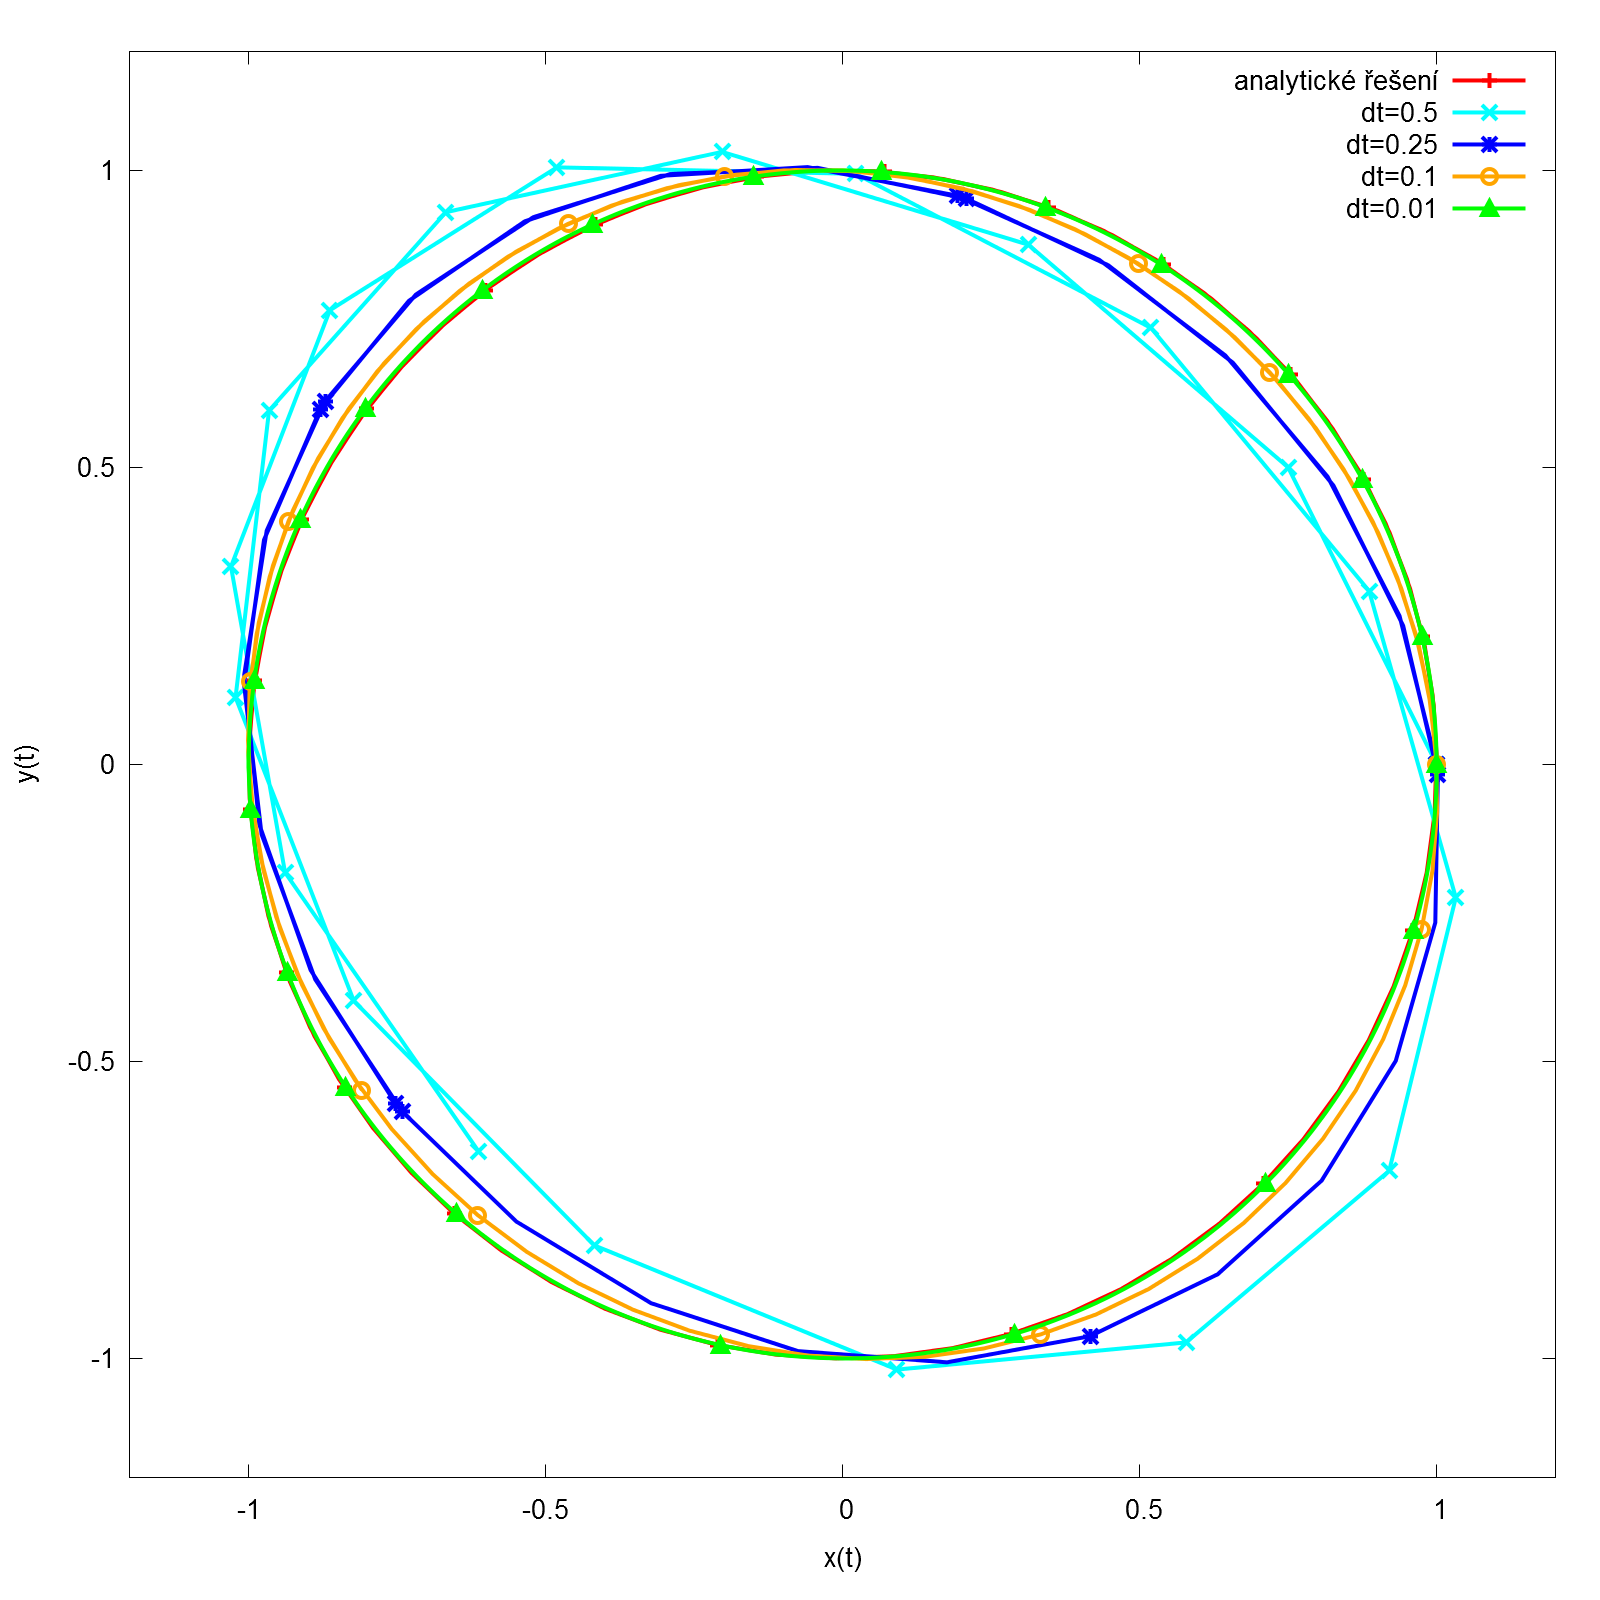
\includegraphics[width=\linewidth]{Figs/semiImplEuler}
\end{figure}
\begin{figure}
	\caption{Semi-implicitní Eulerova metoda $ t\in [0,100] $}
	\label{fig:semiImplEulerStab} 
	\centering
	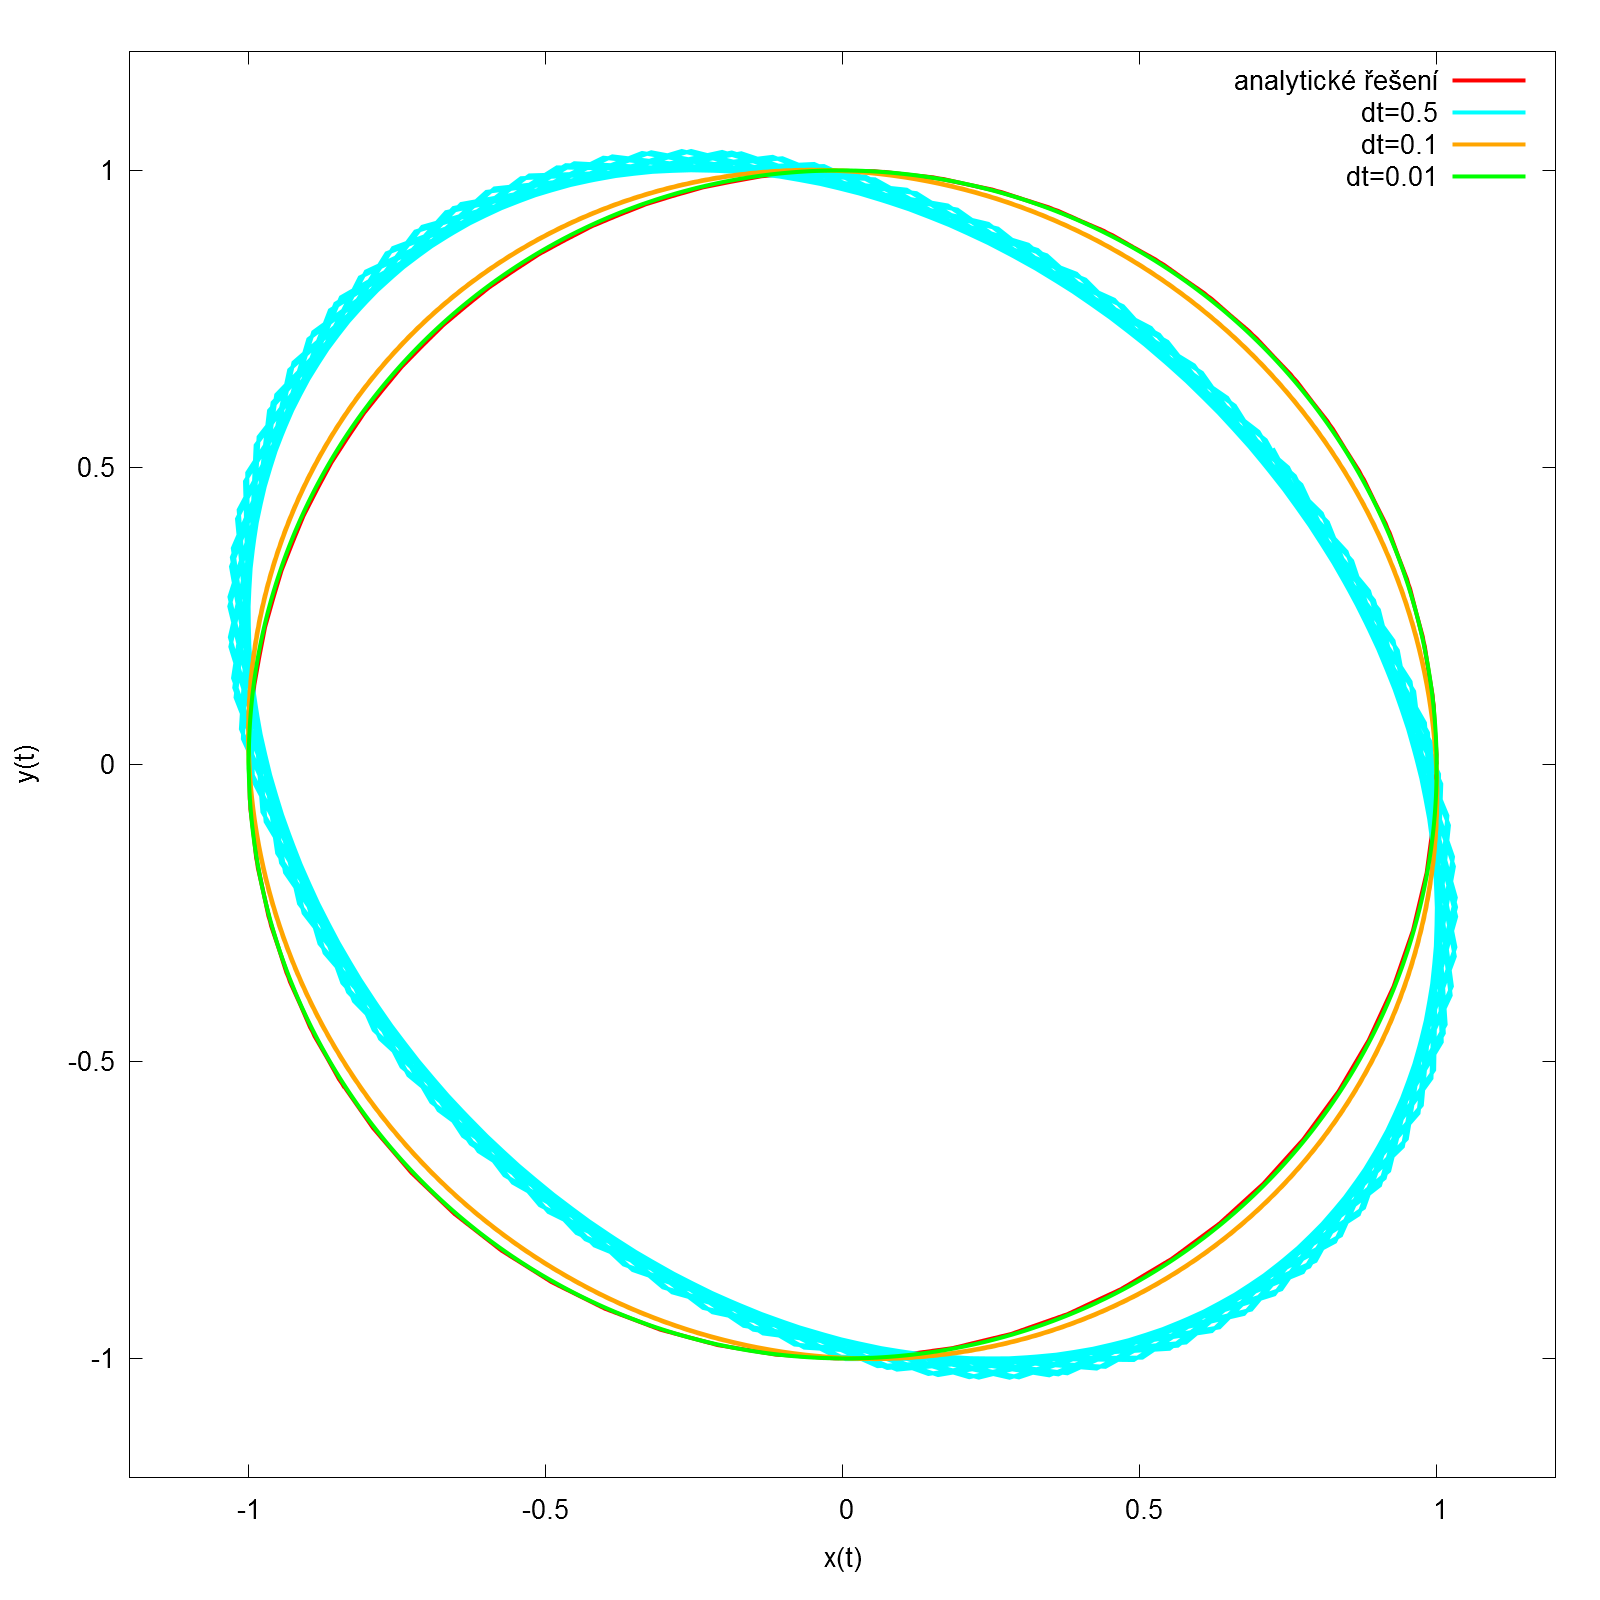
\includegraphics[width=\linewidth]{Figs/semiImplEulerStab}
\end{figure}
\subsection{RK4}
Poslední implementovaná metoda je RK4, která je popsána v sekci \ref{sec:implRK4}. Její přesnost zachycují obrázky \ref{fig:RK4} a \ref{fig:RK4Stab}. Tedy už při $ \Delta t=0.1 $ se jedná o velmi stabilní metodu a je přesnější než semi-implicitní metoda . Ale naopak pro vyšší  $ \Delta t$ stabilní není.
\begin{figure}
	\caption{RK4 metoda $ t\in [0,10] $}
	\label{fig:RK4} 
	\centering
	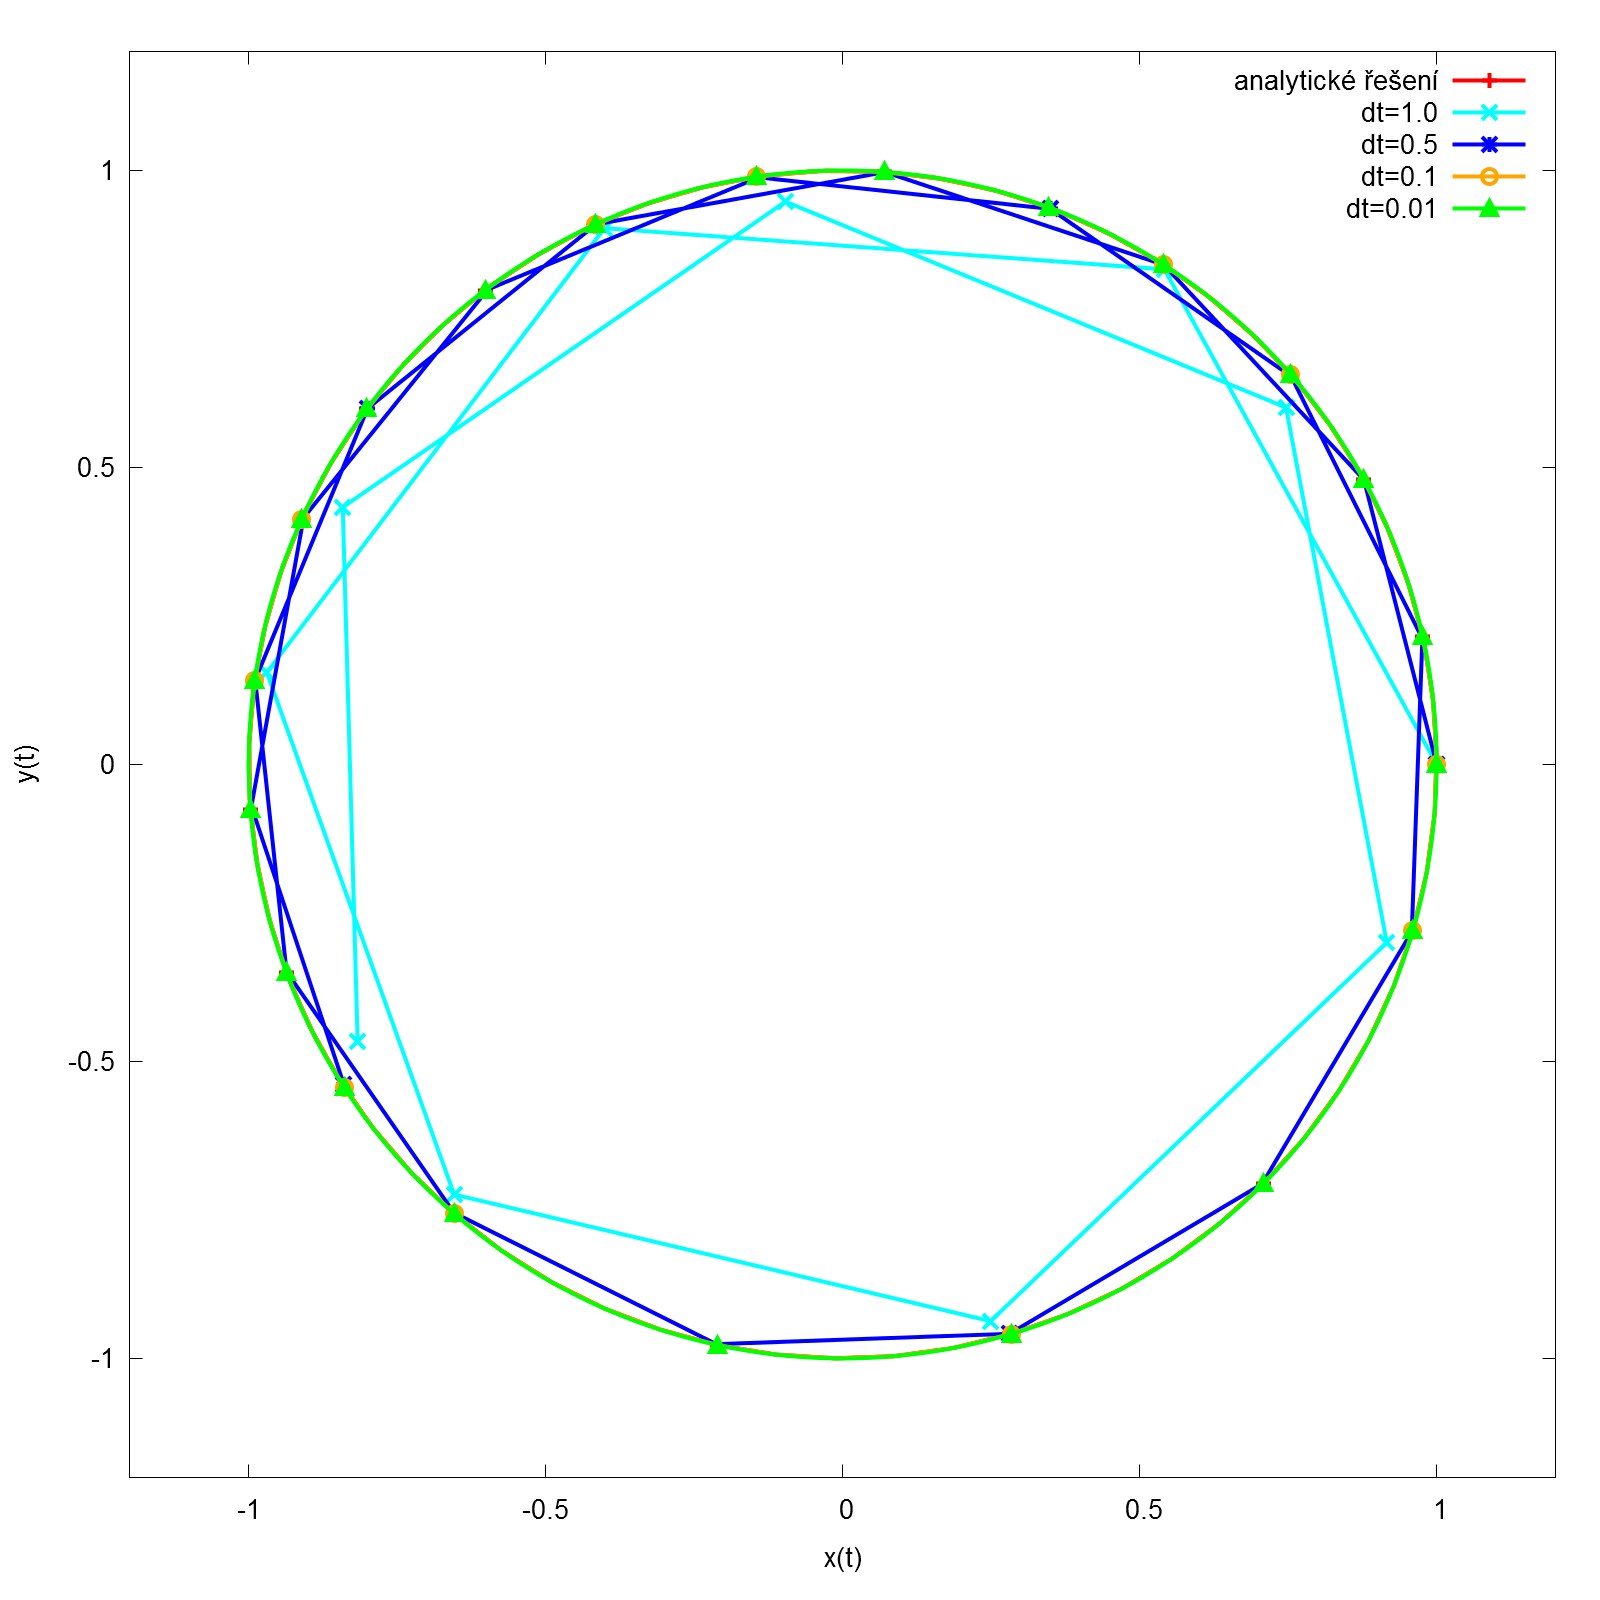
\includegraphics[width=\linewidth]{Figs/RK4}
\end{figure}
\begin{figure}
	\caption{RK4 metoda $ t\in [0,10] $}
	\label{fig:RK4Stab} 
	\centering
	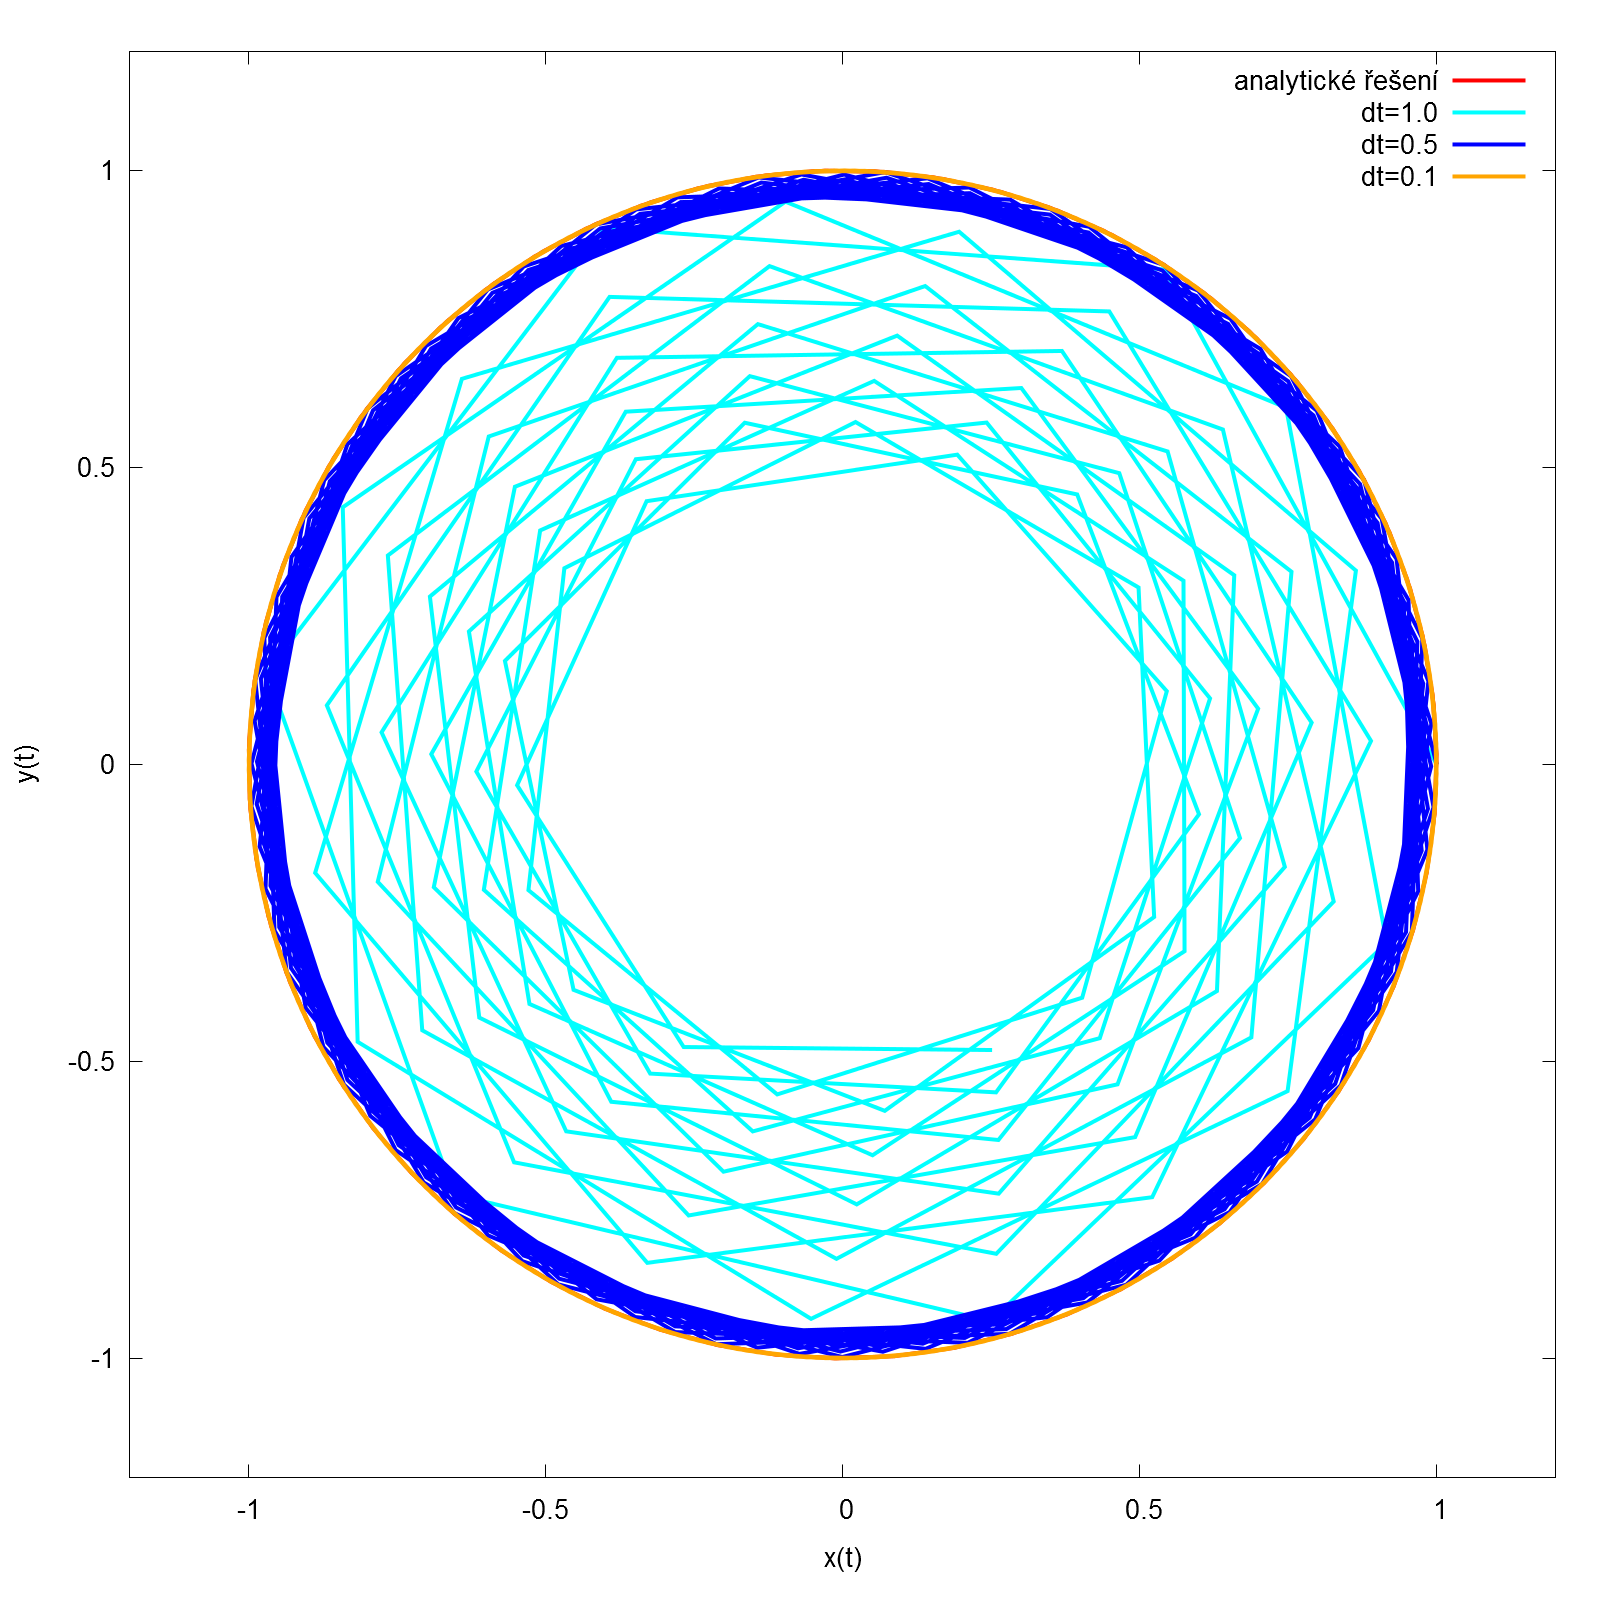
\includegraphics[width=\linewidth]{Figs/RK4Stab}
\end{figure}
\section{Sluneční soustava}
Pojďme se ještě podívat na srovnání stability semi-implicitní a RK4 metody na příkladu naší Sluneční soustavy. Jako indikátor stability použijeme stabilitu oběžných drah měsíců, protože ty mají nejkratší oběžné doby a nestabilita se zde projeví jako první. Samozřejmě toto je pouze nutná a ne postačující podmínka správné simulace, ale pro běžné porovnání by mohla stačit. Naměřené údaje jsou uvedeny v tabulce \ref{tab:stab}. Vyšší hodnoty nejsou podstatné, protože se zde ve velké míře projeví nepřesnost, která vyvolá nestabilitu systému. Každopádně to ukazuje, že semi-implicitní Eulerova metoda je stabilnější, což i trochu naznačovaly obrázky u kruhového pohybu, ale také obrázek \ref{fig:semiImplEulerStab} ukazuje stabilní, avšak nesprávný \uv{orbit}. Na druhou stranu obrázek \ref{fig:RK4Stab} uvádí RK4 jako přesnější metodu pro podobné $ \Delta t $. Přesnost se bohužel pro Sluneční soustavu nedá nijak jednoduše ověřit. 


\arrayrulewidth 1pt
\begin{table}[h]
	\centering
	\label{tab:stab}
	\caption{Stabilita měsíců pro semi-implicitní Eulerovu a RK4 metodu}
	\rowcolors{3}{gray!25}{white}
\begin{tabular}{l  *{8}{|c c} }
	\hline
	 &\multicolumn{2}{c}{Měsíc}&\multicolumn{2}{c}{Phobos}&\multicolumn{2}{c}{Deimos}&\multicolumn{2}{c}{Io}&\multicolumn{2}{c}{Europa}&\multicolumn{2}{c}{Ganymed}&\multicolumn{2}{c|}{Callisto}&\multicolumn{2}{c}{\textbf{Celkem}}\\\hline
	DTmult &S&R&S&R&S&R&S&R&S&R&S&R&S&R&S&R\\\hline
	70 000&
	\cmark&\cmark&\cmark&\cmark&\cmark&\cmark&\cmark&\cmark&\cmark&\cmark&\cmark&\cmark&\cmark&\cmark&
	\textbf{7}&\textbf{7}\\
	80 000&
	\cmark&\cmark&\cmark&\xmark&\cmark&\cmark&\cmark&\cmark&\cmark&\cmark&\cmark&\cmark&\cmark&\cmark&
	\textbf{7}&\textbf{6}\\
	300 000&	
	\cmark&\cmark&\cmark*&\xmark&\cmark&\cmark&\cmark&\cmark&\cmark&\cmark&\cmark&\cmark&\cmark&\cmark&
	\textbf{7}&\textbf{6}\\
	320 000&	
	\cmark&\cmark&\xmark&\xmark&\cmark&\xmark&\cmark&\cmark&\cmark&\cmark&\cmark&\cmark&\cmark&\cmark&
	\textbf{6}&\textbf{5}\\
	400 000&	
	\cmark&\cmark&\xmark&\xmark&\cmark&\xmark&\cmark&\xmark&\cmark&\cmark&\cmark&\cmark&\cmark&\cmark&
	\textbf{6}&\textbf{4}\\
	1 000 000&	
	\cmark&\cmark&\xmark&\xmark&\cmark&\xmark&\cmark&\xmark&\cmark&\xmark&\cmark&\cmark&\cmark&\cmark&
	\textbf{6}&\textbf{3}\\
	1 200 000&	
	\cmark&\cmark&\xmark&\xmark&  \cmark**&\xmark&\cmark&\xmark&  \xmark**&\xmark&  \xmark**&\cmark&\cmark&\cmark&
	\textbf{4}&\textbf{3}\\
	1 300 000&	
	\cmark&\cmark&\xmark&\xmark&\xmark&\xmark&\xmark&\xmark&\xmark&\xmark&\cmark&\cmark&\cmark&\cmark&
	\textbf{3}&\textbf{3}\\
	\hline
\end{tabular}
	\newline
	\flushleft
	\textit{S=semi-implicitní; R=RK4 metoda. Krok simulace byl $ DTmult*10 $ms.\\ Stabilita znamená, že měsíc stále obíhal kolem své planety po 5/20/60 letech simulovaného času pro $ DTmult \geq0 /\geq3.10^5/\geq10^6 $ . Tabulka neobsahuje všechny hodnoty, pouze ty, kolem kterých došlo ke změnám.\\
	*Phobos opisuje 13-úhelník, ale je stabilní.\\
	**Ganyméd a Europa se nejspíše srazily, Deimos stabilně opisuje 12-úhelník.}
\end{table}
\section{Rychlosti a Závěr}
Srovnání rychlostí obou metod nabízí tabulka \ref{tab:rychlost}. 

Z tabulky plyne, že RK4 je přibližně 3-4x pomalejší než Eulerova metoda. Takže ve výsledku je dle našich měření RK4 pomalejší a nestabilnější, přesto je použita jako výchozí. Důvod je ten, že je podle mne mnohem přesnější, stabilita Eulera vypadá sice dobře, ale silně pochybuji, že v tu chvíli simulace odpovídá realitě. Ale samozřejmě uživatel si může stále vybrat, což byl také účel a tato kapitola měla za cíl toto rozhodnutí alespoň trochu ulehčit. Takže pokud chce spíše stabilní, avšak možná nepřesnou simulaci, tak je lepší Eulerova metoda, pokud dává přednost přesnosti, tak bych volil RK4 nebo jiné. Bohužel \uv{jiné} zde nejsou, což je škoda a proto je to také jedno z možných rozšíření viz. \ref{sec:vylepseni}.
\begin{table}
	\centering
	\label{tab:rychlost}
	\caption{Srovnání rychlostí semi-implicitní Eulerovy a RK4 metody}
	\rowcolors{3}{gray!25}{white}
	\begin{tabular}{l l c c c}
		\hline\multicolumn{2}{c}{\multirow{2}{*}{\textbf{Metoda}}}& & \textbf{Počet objektů}\\ 
		&& 10 & 20 & 100\\
		\hline
		Euler&Debug&1ms&2ms&3ms\\
			 &Release&1ms&2ms&3ms\\\hline
		RK4&Debug&1ms&2ms&3ms\\
		&Release&1ms&2ms&3ms\\\hline
	\end{tabular}
	\newline
	\flushleft
	\textit{Přesné nastavení Debug a Release je uvedeno v .sln u zdrojových souborů. Release má zapnuté veškeré optimalizace - inlining, SIMD...;Debug je výchozí režim bez většiny optimalizací. Hodnoty byly vypočteny z 100 000 volání každé funkce na soustavě s procesorem 4320 - 4x3.6Ghz se systémem Win7 64-bit(Ale aplikace je 32-bitová.)}
\end{table}
\section{Závěr}
Proč RK4
	\chapter{Uživatelská příručka}
\label{chap:userGuide}
\section{Požadavky}
Vyžaduje verzi OpenGL 3 nebo vyšší, navíc je potřeba balíček Microsoft Visual C++ 2015 Redistributable, který je ve formě .dll přibalen. Pokud by s ním přesto byly problémy, tak doporučuji stáhnout  a nainstalovat jeho aktuální verzi z \url{https://www.microsoft.com/cs-CZ/download/details.aspx?id=53840}
\section{Základní ovladání}
Při spuštění se program otevře v výchozím grafickém režimu, kde dojde k nahrání zabudované Sluneční soustavy. Simulace se ovládá pomocí grafického rozhraní - Obrázek \ref{fig:GUI1}.\\
\begin{figure}
	\caption{Grafické rozhraní programu}
	\label{fig:GUI1} 
	\centering
	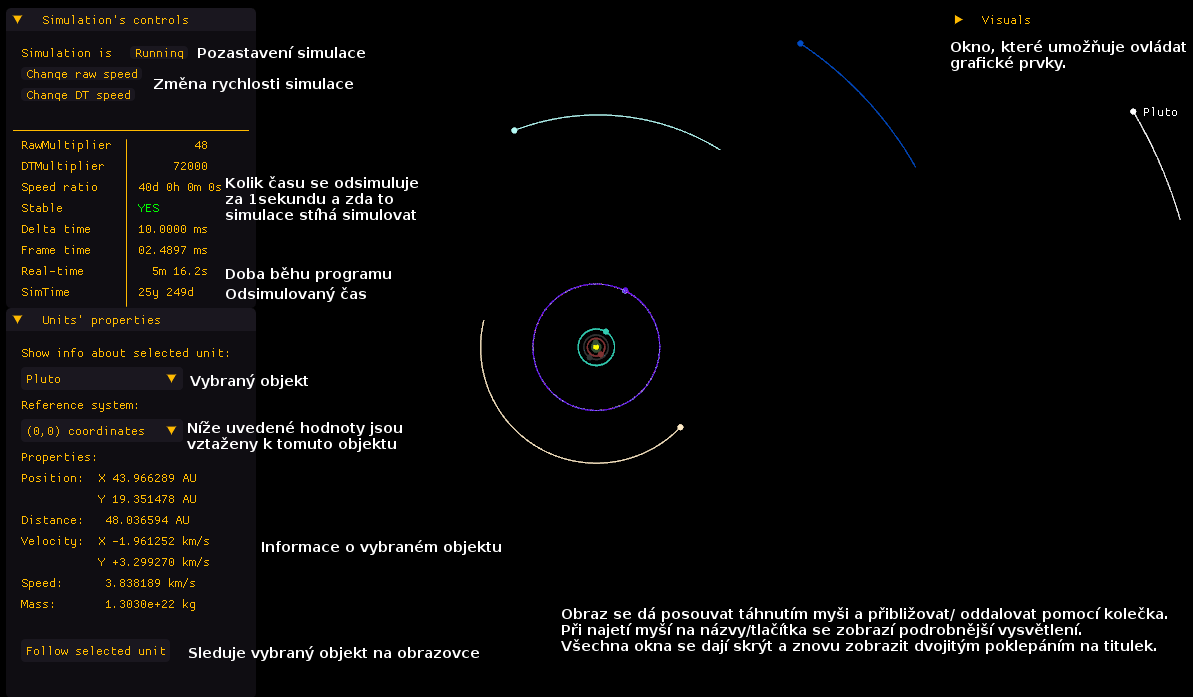
\includegraphics[scale=0.5]{Figs/GUI1_edited}
\end{figure}
\FloatBarrier
\section{Pokročilé možnosti}
Program také nabízí pokročilejší ovládání pomocí příkazové řádky, s níž je možné načítat simulovaná data ze souboru, vybrat si integrační metody a také možnost zaznamenat a následně přehrát uložené simulace.
Pro vypsání nápovědy a všech dostupných příkazů v českém jazyce použijte:
\ \texttt{\textbf{SolarSystem.exe -help -cz}}
\\\\
Uveďme zde alespoň pár dalších příkladů různých příkazů:
\begin{enumerate}
	\item \texttt{\textbf{SolarSystem.exe vstup.txt}} \\
	Načte vstupní data z formátovaného souboru \texttt{vstup.txt} a spustí simulaci, která bude běžet v reálném čase a zobrazovat se v okně 1200x700 s uživatelským rozhraním.
	\item \texttt{\textbf{SolarSystem.exe -sim -p formatted -i vstup.txt -m RK4 -v win}} \\
	 Ekvivalentní zápis předchozího příkladu. S explicitním použitím modulů.
	\item \texttt{\textbf{SolarSystem.exe -sim -rm 24 -dm 3600 -x 300}} \\
	Spustí podobnou simulaci jako v 1. příkladu. Akorát bude mít 3600x větší integrační krok a bude probíhat 10x rychleji. Ve výsledku se tedy odsimuluje jeden den za jednu reálnou sekundu. Simulace se vypne po 5 minutách běhu.
	\item \texttt{\textbf{SolarSystem.exe -record -r zaznam.replay -p formatted -i vstup.txt -o vystup.txt -m semiEuler -rm 24 -dm 3600 -x 60}}\\
	Zaznamená 60 sekundovou simulaci do souboru \texttt{zaznam.replay}, vstupní data načte z formátovaného souboru \texttt{vstup.txt} a výsledná data uloží do \texttt{vystup.txt} ve stejném formátu. Simulace bude simulovat jeden den za jednu sekundu pomocí semi-implicitní Eulerovy integrační metody. Simulace se spustí v grafickém prostředí stejně jako v 1. příkladě.
	\item  \texttt{\textbf{SolarSystem.exe zaznam.replay}}\\
	Přehraje zaznamenanou simulaci z předchozího příkladu v grafickém prostředí.
\end{enumerate}
K .exe souboru je přiložen vzorový formátovaný text \texttt{vstup.txt} a také jeden záznam simulace \texttt{zaznam.replay}.
Přesný popis formátovaného vstupního souboru je uveden v sekci \ref{sec:strukturaDat} . Pro detailní vysvětlení parametrů simulace je k dispozici popis v sekci \ref{sec:startMetoda}.


\chapter{Kompilace programu}
\label{chap:kompilace}
\section{Git}
Tato dokumentace spolu se zdrojovými kódy programu je veřejně dostupná na:
\begin{center}
\texttt{https://bitbucket.org/Quimby/solar/src}
\end{center}
Popřípadě přímo stažitelná pomocí git HTTPS\eqref{git:https} nebo SSH\eqref{git:ssh}:
\begin{align}
	\label{git:https}
	\texttt{https://Quimby@bitbucket.org/Quimby/solar.git}\\
	\label{git:ssh}
	\texttt{git@bitbucket.org:Quimby/solar.git}
\end{align}
\section{Windows}
Program byl tvořen v programu Visual Studio 2015 Community Edition, takže je zde už předpřipravený .sln projekt, který by měl obsahovat vše potřebné pro správné zkompilování.
\section{Linux}
Program by zde měl být teoreticky také plně funkční, avšak není zde zatím žádný pomocný projekt ani makefile. Kdyžtak je potřeba nejdříve stáhnout a zkompilovat externí knihovny - GLFW, GLEW. Návod by měl být na jejich oficiálních stránkách . Momentálně obě knihovny nabízí vytvoření potřebných souborů pomocí programu CMake, takže kompilace by neměla být těžká. Dále kompilace samotného programu vyžaduje minimálně flag \texttt{GLEW\_STATIC} a také include path do složky obsahující složku \texttt{Source/}(defaultně se nachází ve složce SolarSystem) a samozřejmě slinkovat obě knihovny, ale pak by už mělo vše fungovat. 

	
\end{document}